\documentclass[9pt]{article}
\usepackage[spanish]{babel}
\usepackage[utf8]{inputenc}
\usepackage{graphicx}
\graphicspath{{media/}}
\usepackage{float}
\usepackage{caption}
\captionsetup{labelformat=empty}
%\renewcommand{\familydefault}{\sfdefault}
\title{Proyecto 1}
\author{Carlos Gerardo Acosta Hernández \\ Andrea Itzel González Vargas \\ Luis Pablo Mayo Vega}
\date{Redes de Computadoras\\Facultad de Ciencias, UNAM}
\setlength{\parindent}{0em}
\begin{document}
\maketitle

\section*{Reporte}

\subsection*{Diagrama de Red}
\begin{figure}[ht!]
  \centering
  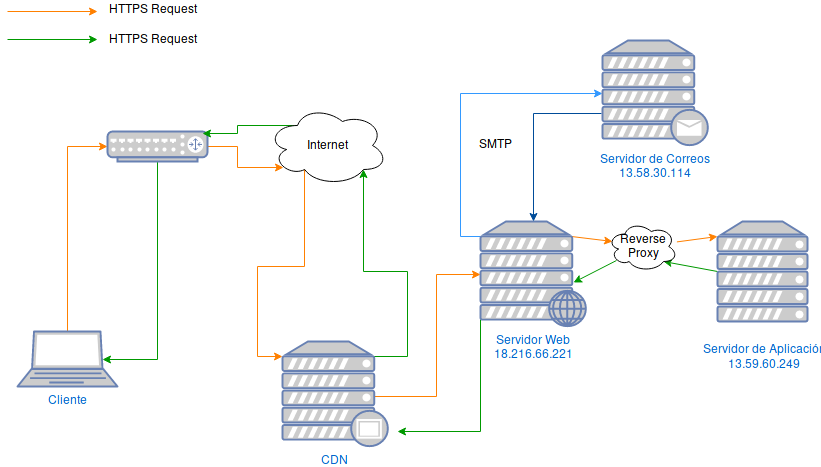
\includegraphics[width=\textwidth]{net_diagram}
  \caption{Diagrama de red de los servidores web, de aplicación y de correo electrónico}
\end{figure}
\subsection*{DNS}
El servicio de \textsf{DNS} que utilizamos es \textsf{Route 53} de Amazon, pues está integrado en la misma plataforma que los servidores y al ser diseñado para trabajar en conjunto, la integración fue mucho más fácil que con Cloudflare.
\begin{figure}[H]
  \centering
  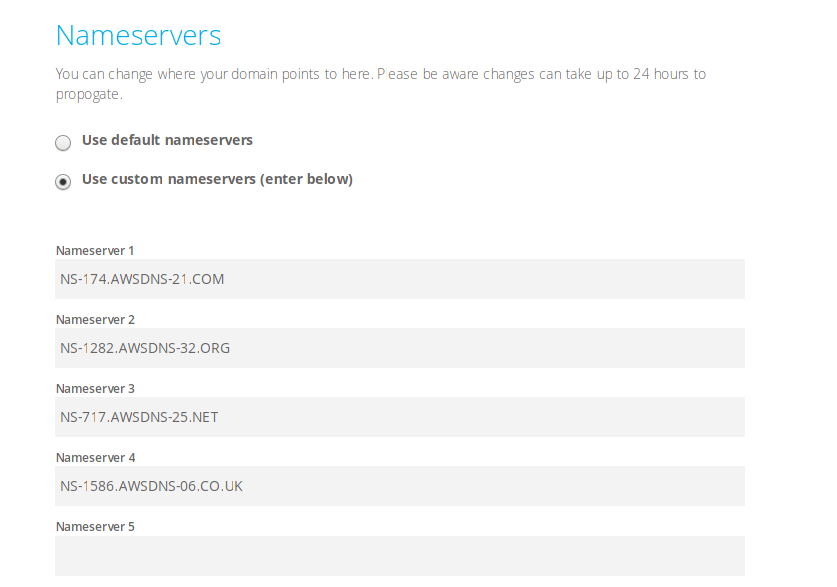
\includegraphics[width=\textwidth]{nameservers}
  \caption{Nameservers de Amazon agregados en la configuración de freenom}
\end{figure}
\begin{figure}[H]
  \centering
  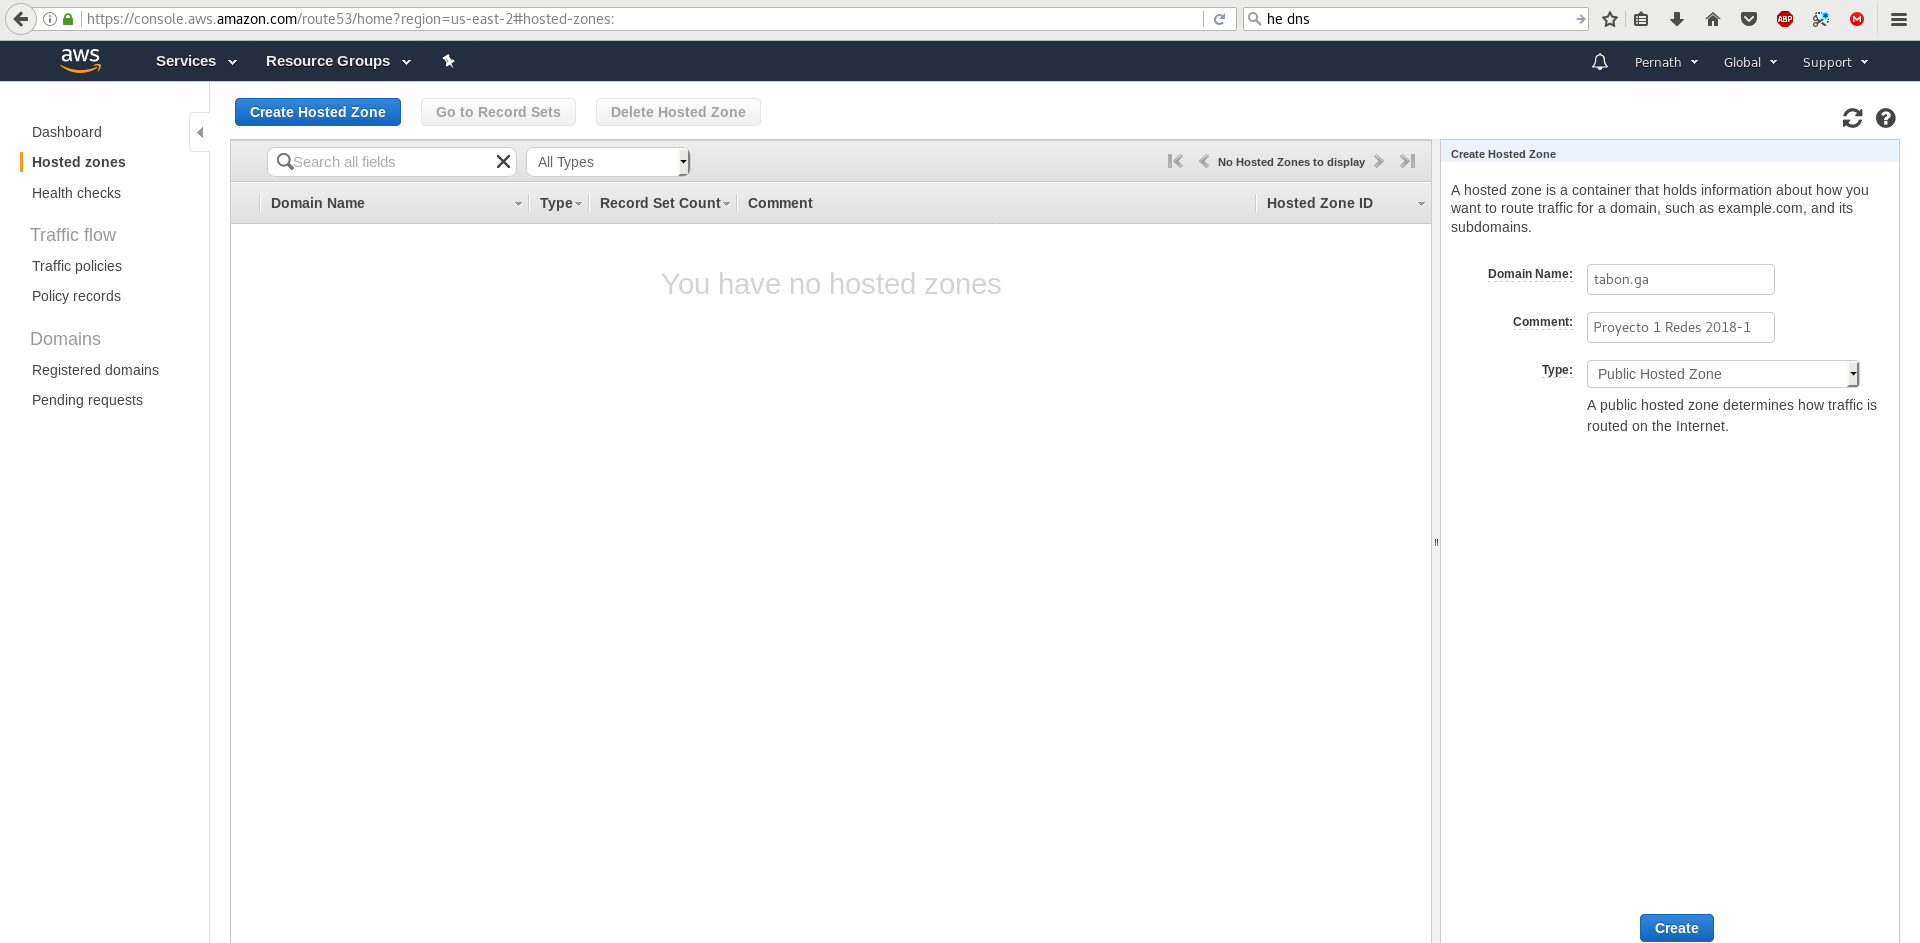
\includegraphics[width=\textwidth]{DNS_management}
  \caption{Panel de control de Route 53 sin zonas creadas}
\end{figure}
\begin{figure}[H]
  \centering
  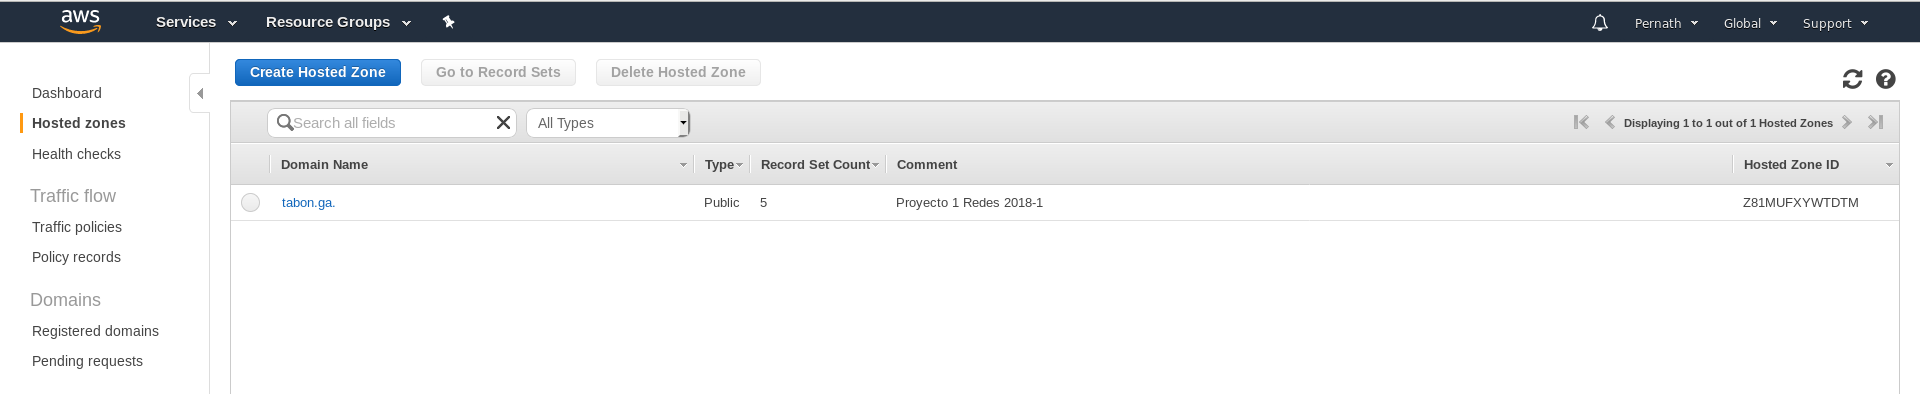
\includegraphics[width=\textwidth]{HostedZones}
  \caption{zonas creadas}
\end{figure}
\begin{figure}[H]
  \centering
  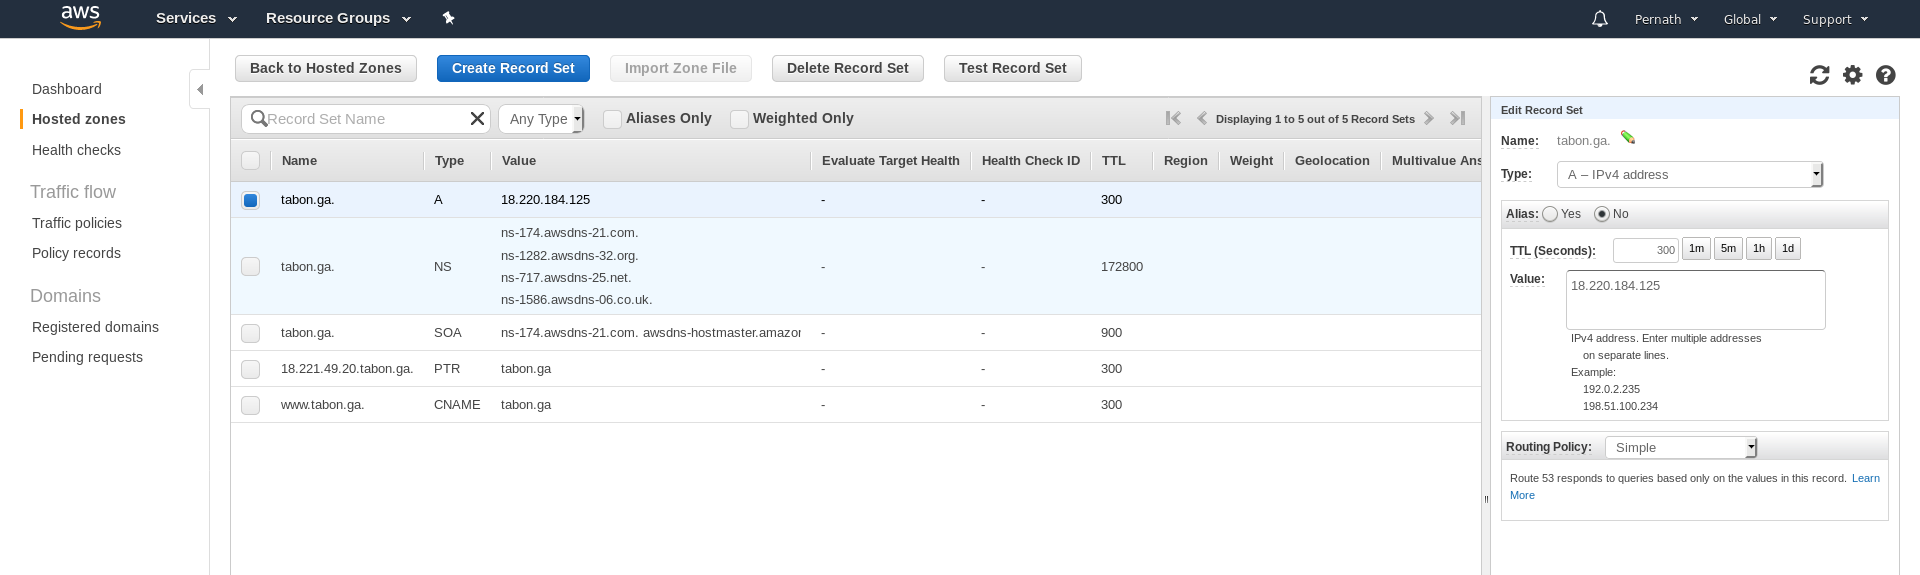
\includegraphics[width=\textwidth]{A}
  \caption{Detalles del registro A para IPv4}
\end{figure}
\begin{figure}[H]
  \centering
  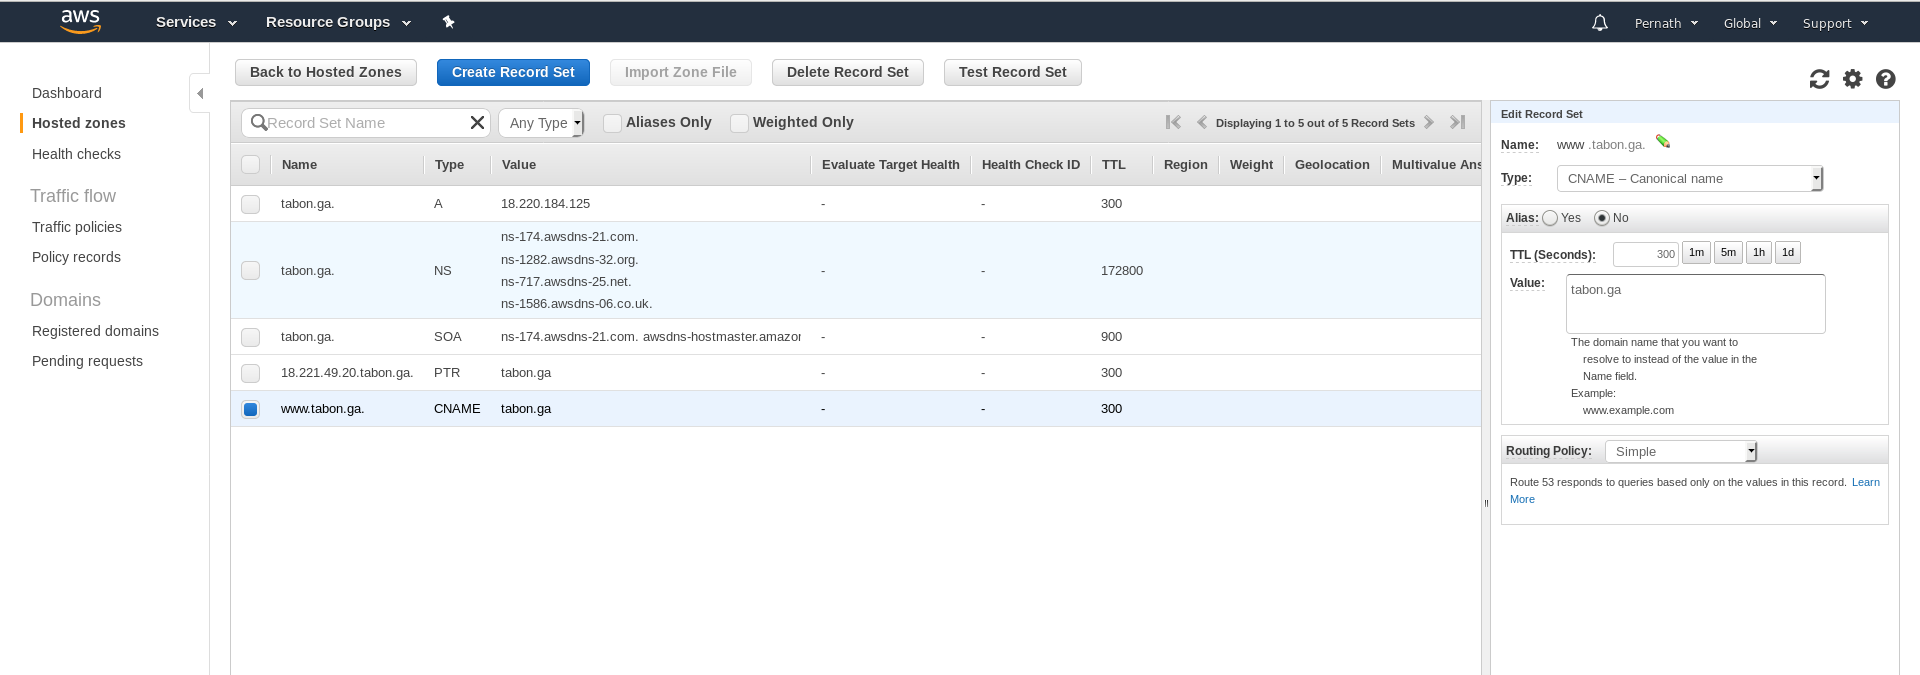
\includegraphics[width=\textwidth]{CNAME}
  \caption{Detalles del registro CNAME para nombre canónico}
\end{figure}
\begin{figure}[H]
  \centering
  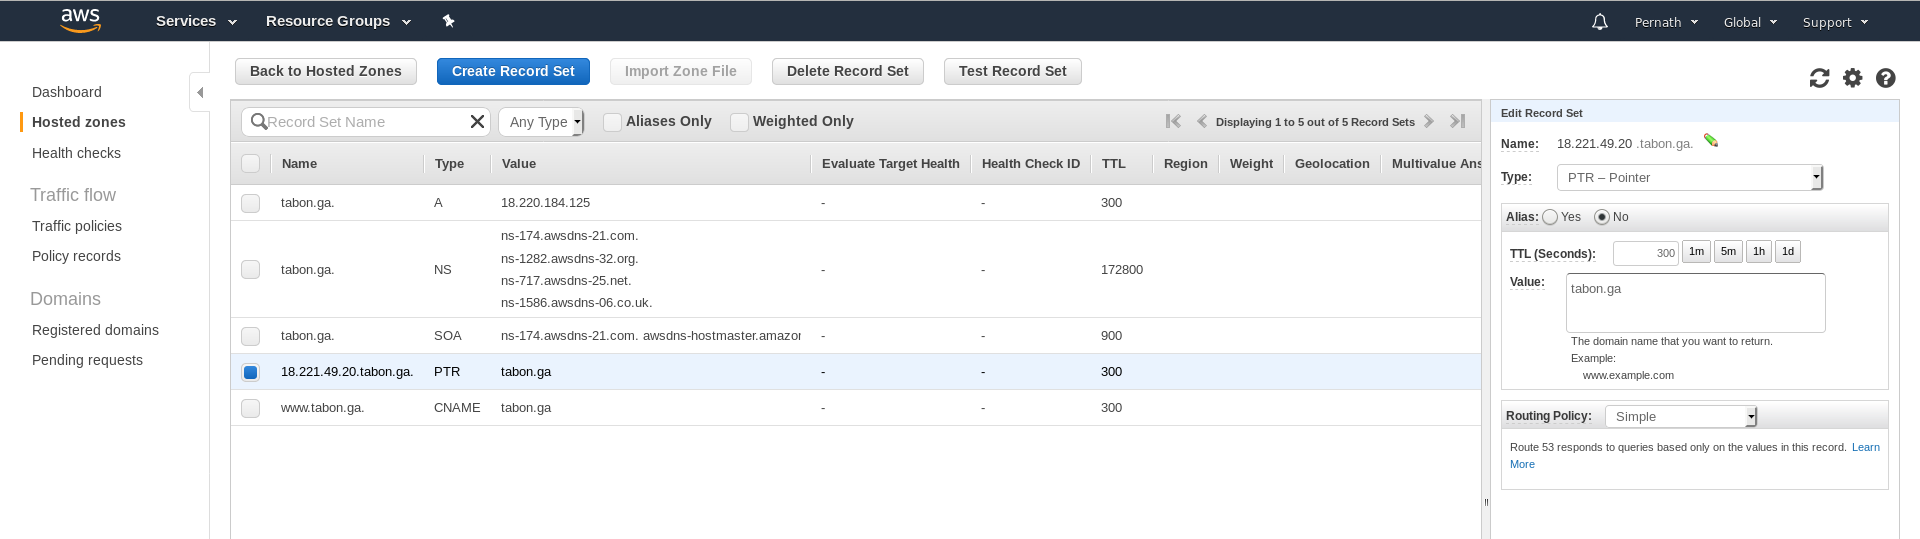
\includegraphics[width=\textwidth]{PTR}
  \caption{Detalles del registro PTR}
  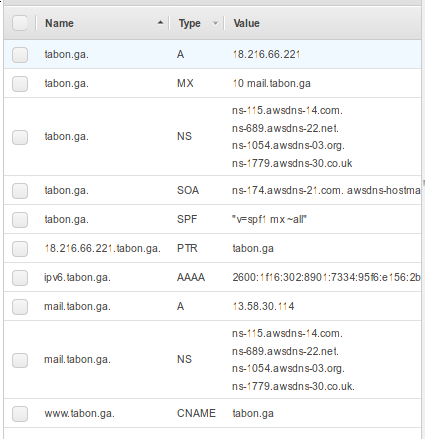
\includegraphics[width=\textwidth]{record_set}
  \caption{Vista de todos los registros}
\end{figure}

\subsection*{Resumen de las configuraciones del servidor web y el servidor de aplicación y base de datos}
Se usaron 3 instancias de la plataforma \textsf{EC2} de Amazon  para los servidores de la aplicación, cada una con la distribución \textsf{Ubuntu 16.04} y con manejo a través de \textsf{ssh}. También se obtuvieron certificados para el cifrado en el protocolo \textsf{TLS} para el acceso mediante \textsf{HTTPS} al sitio. 
\begin{figure}[H]
  \centering
  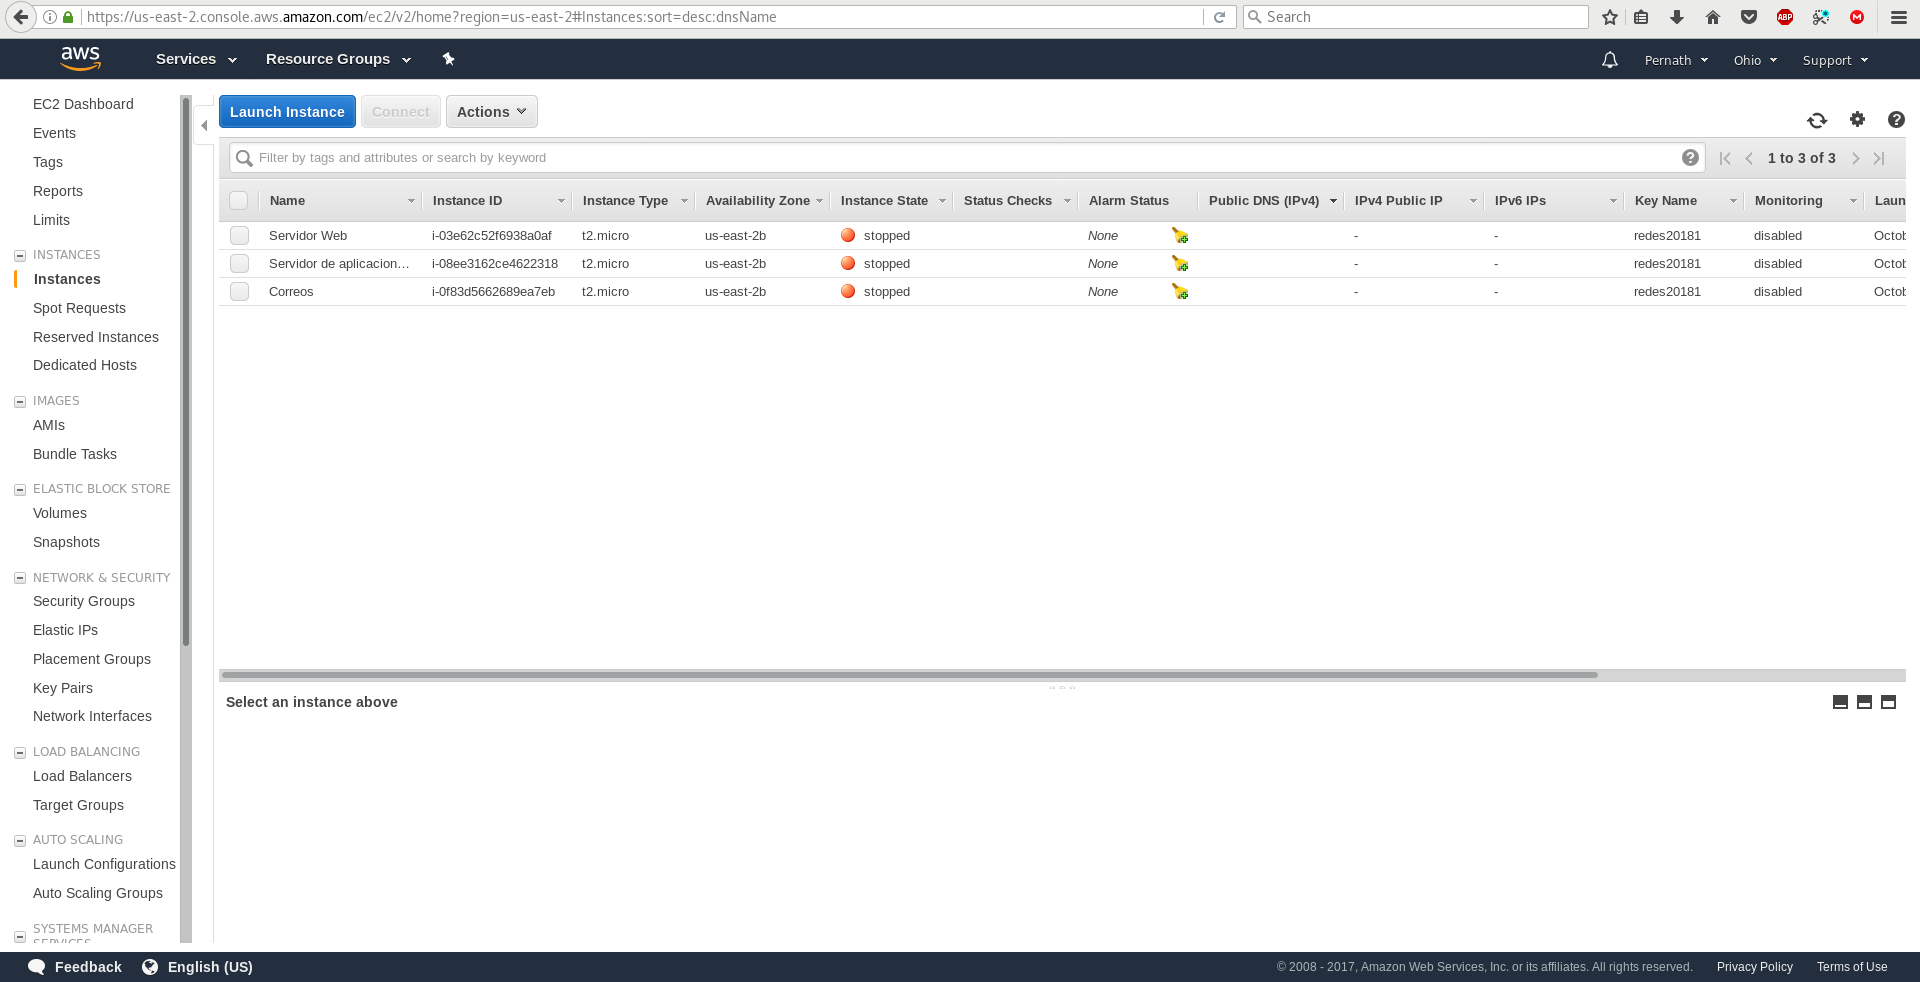
\includegraphics[width=\textwidth]{instances_dashboard}
  \caption{panel de control de las VPC}
\end{figure}
\begin{figure}[H]
  \centering
  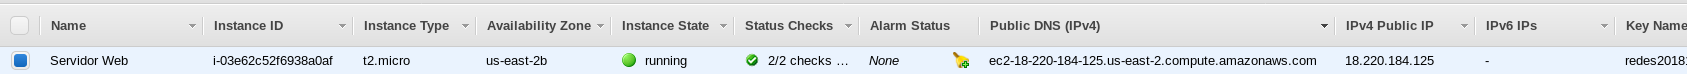
\includegraphics[width=\textwidth]{web_server}
  \caption{Servidor web en ejecución}
\end{figure}

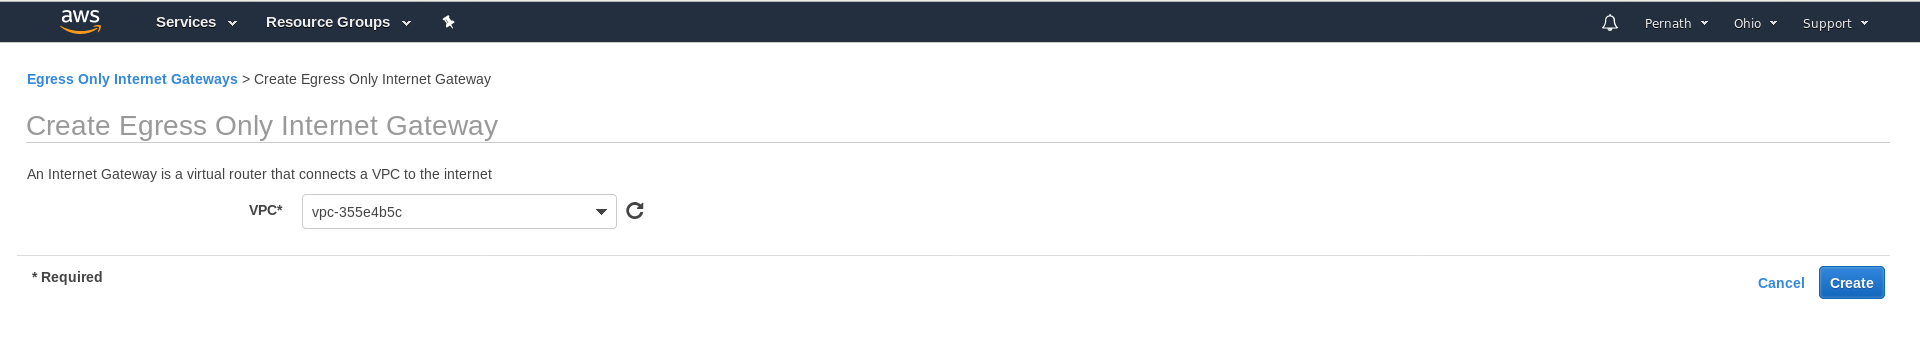
\includegraphics[width=\textwidth]{egress_only_gateway}
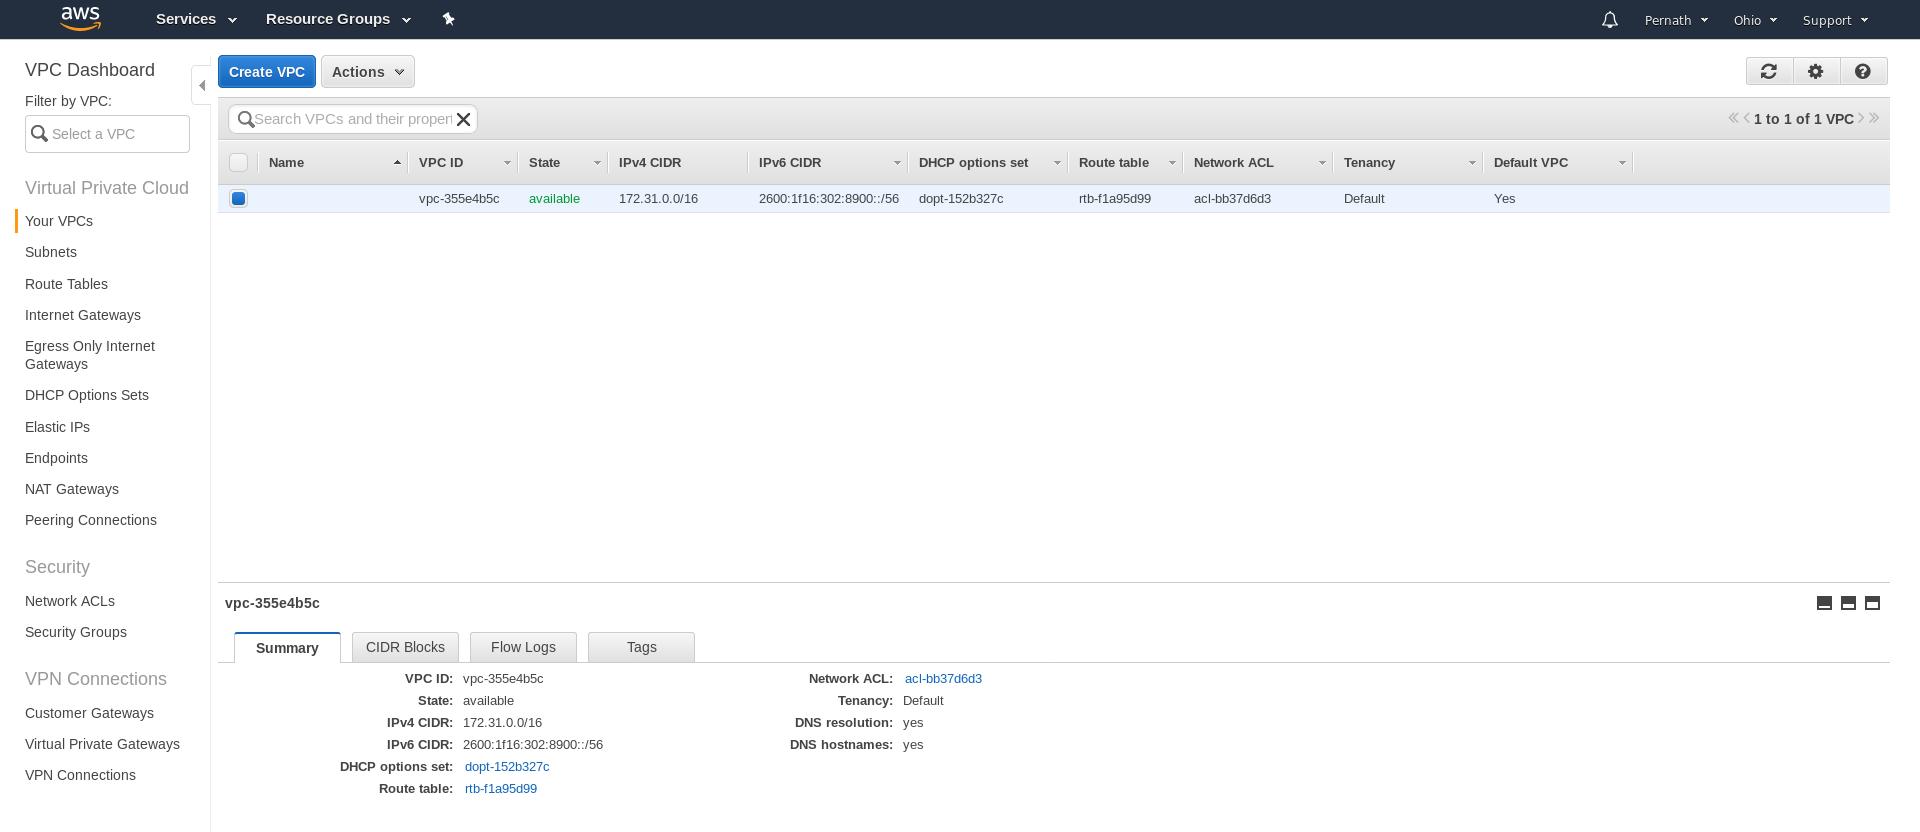
\includegraphics[width=\textwidth]{vpc}
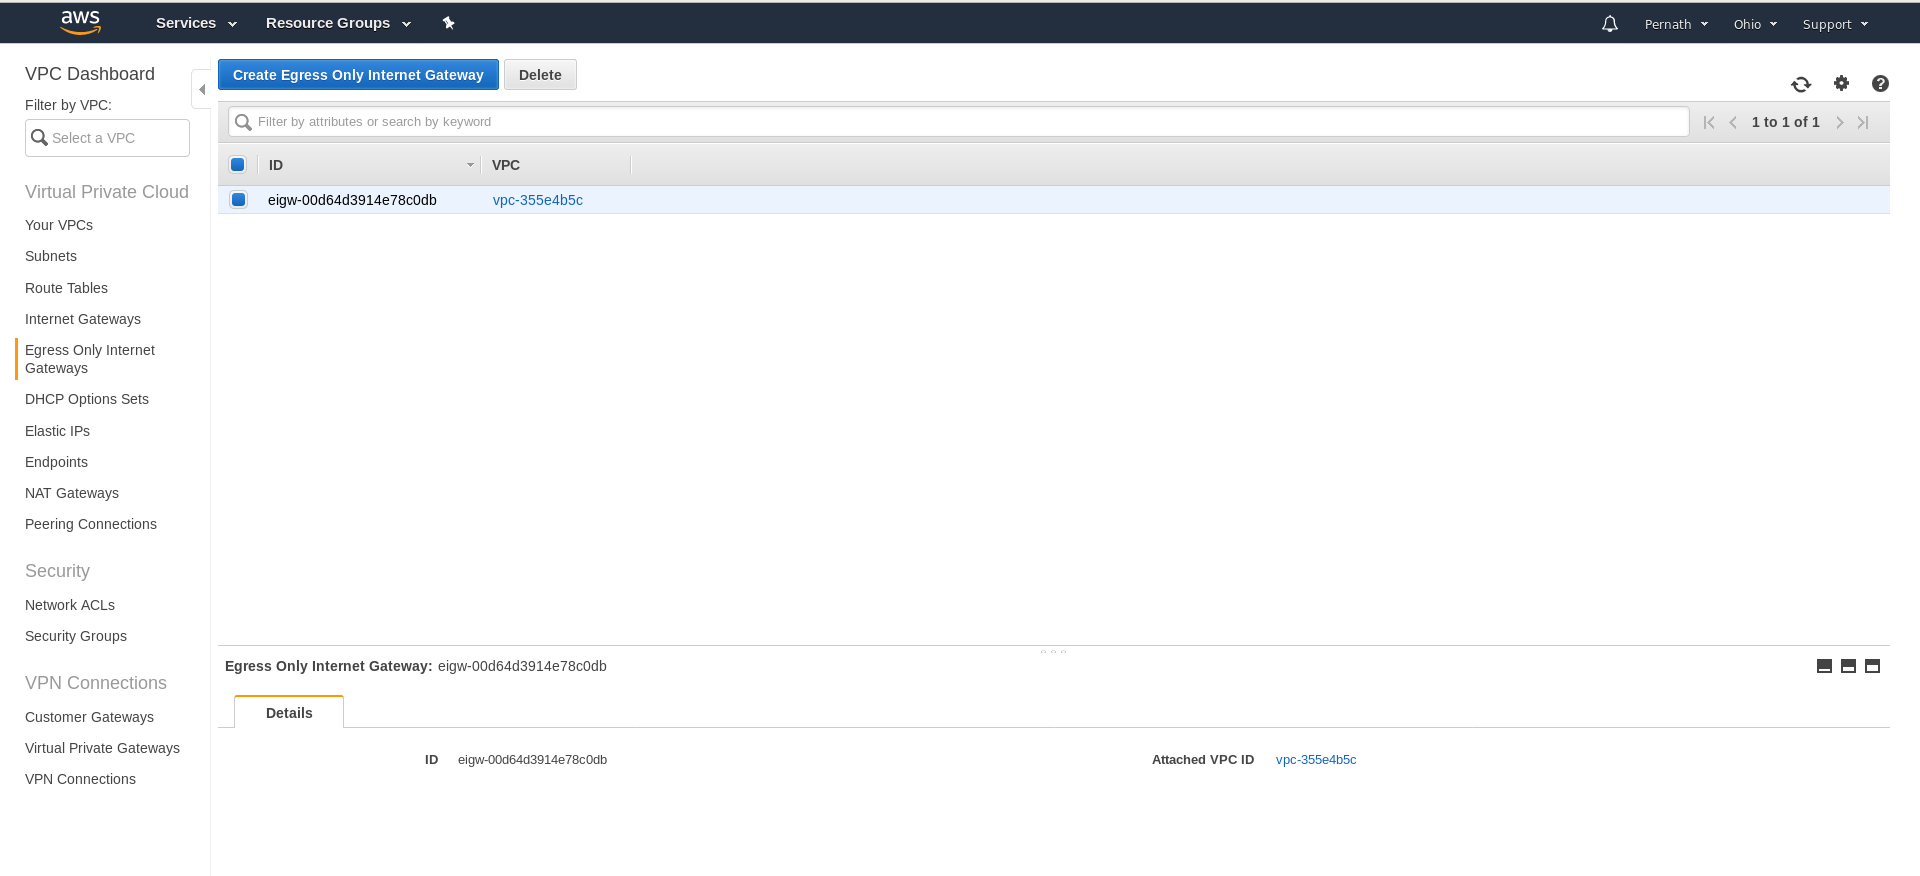
\includegraphics[width=\textwidth]{vpc_egress_only}
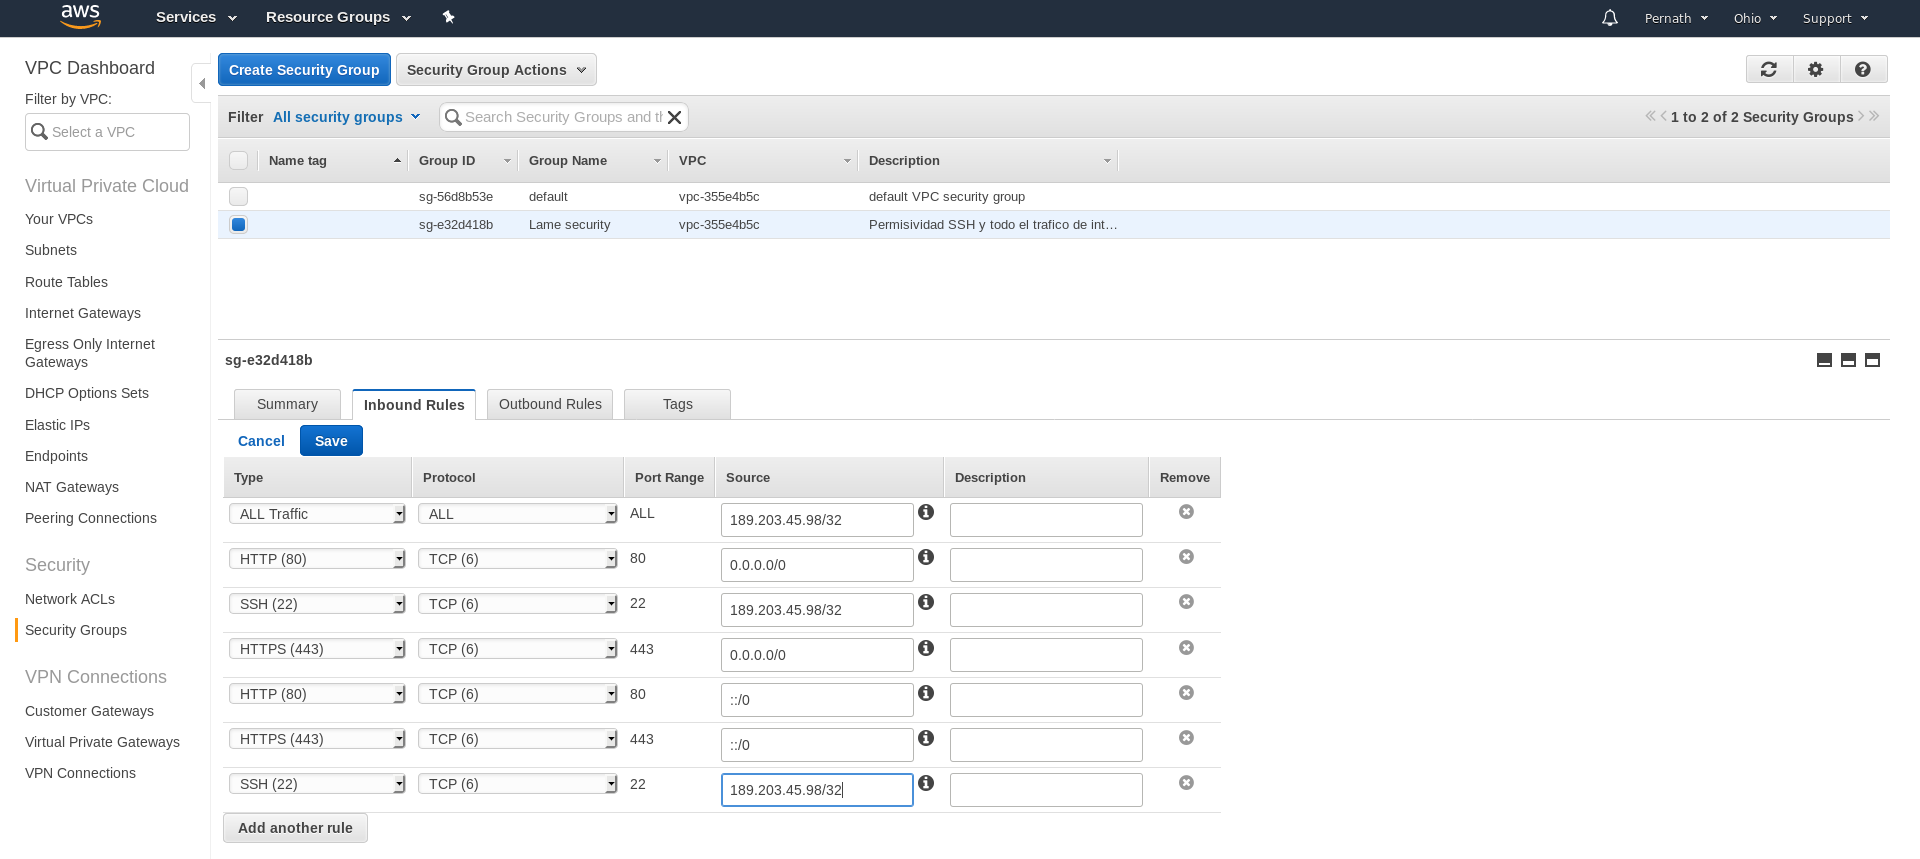
\includegraphics[width=\textwidth]{edit_security_group}
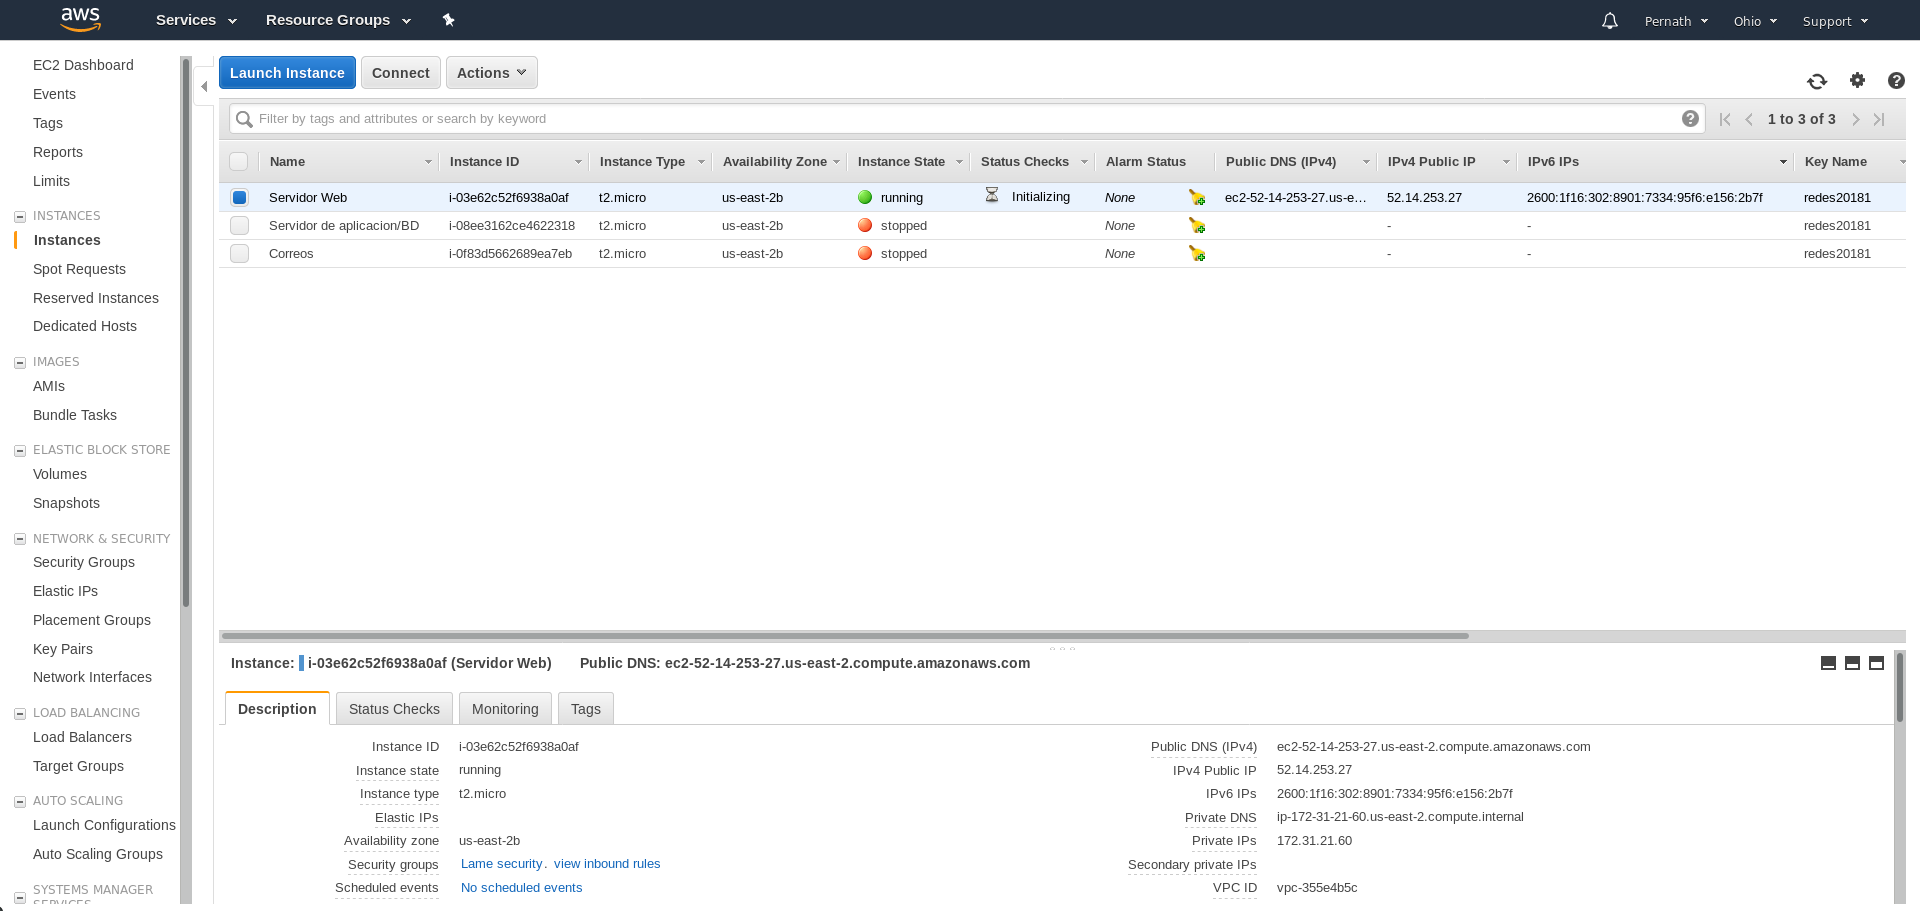
\includegraphics[width=\textwidth]{ipv6_assignment}
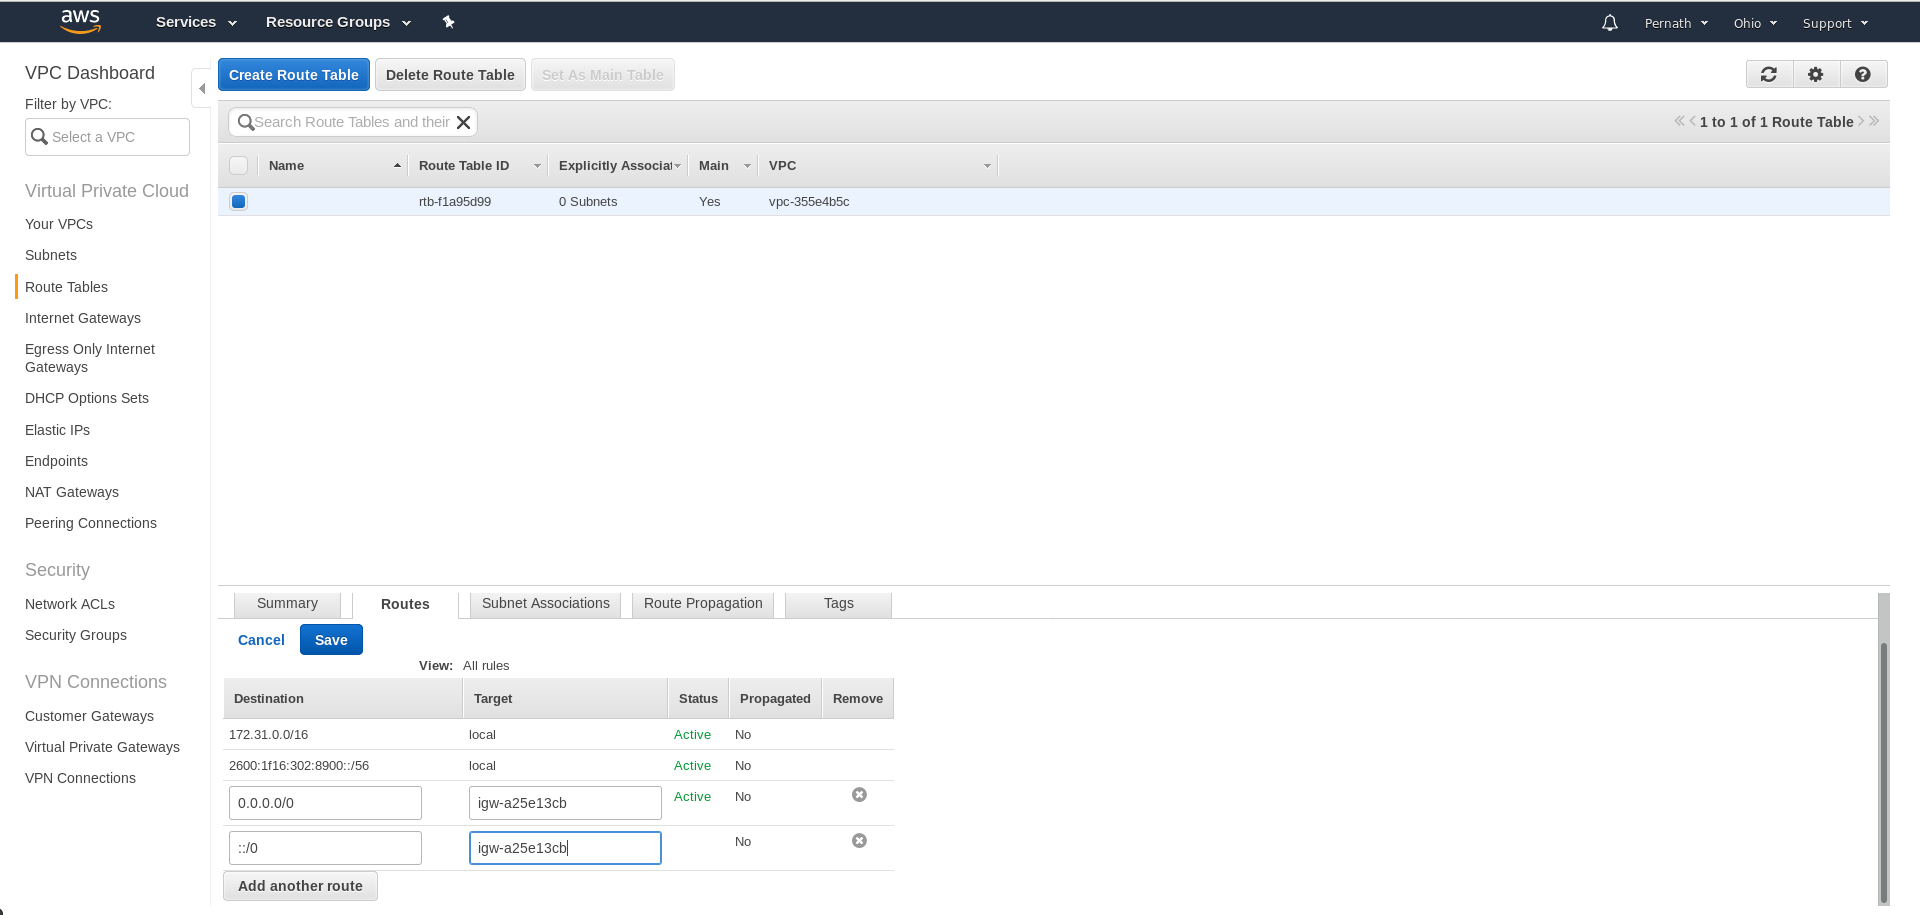
\includegraphics[width=\textwidth]{public_subnet}
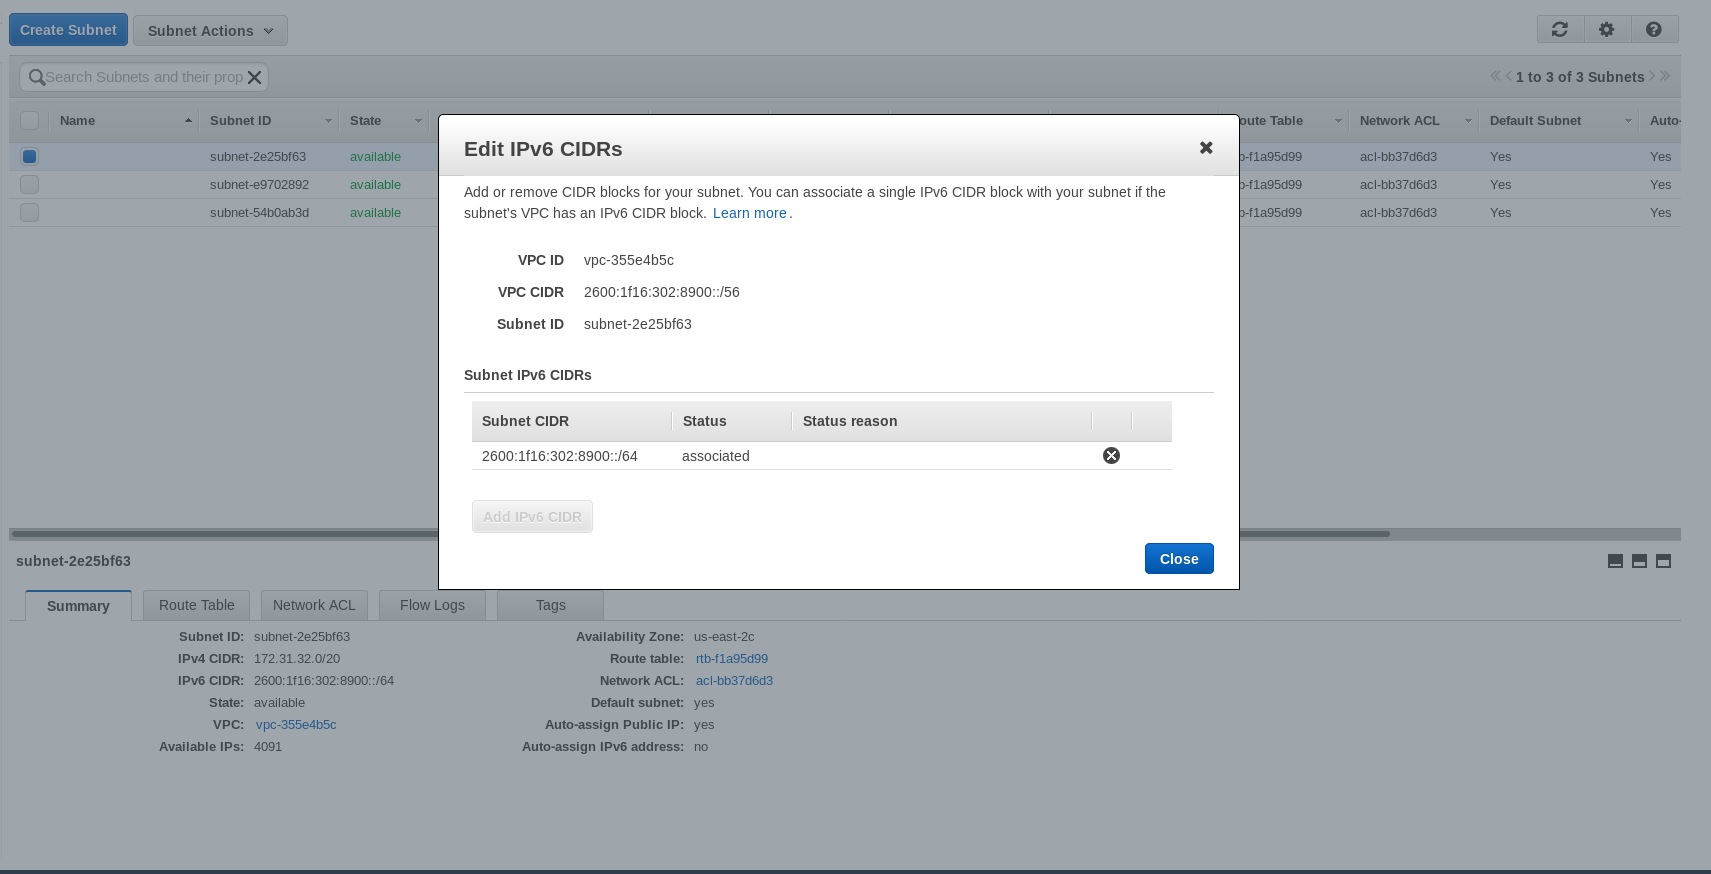
\includegraphics[width=\textwidth]{ipv6_cidr}
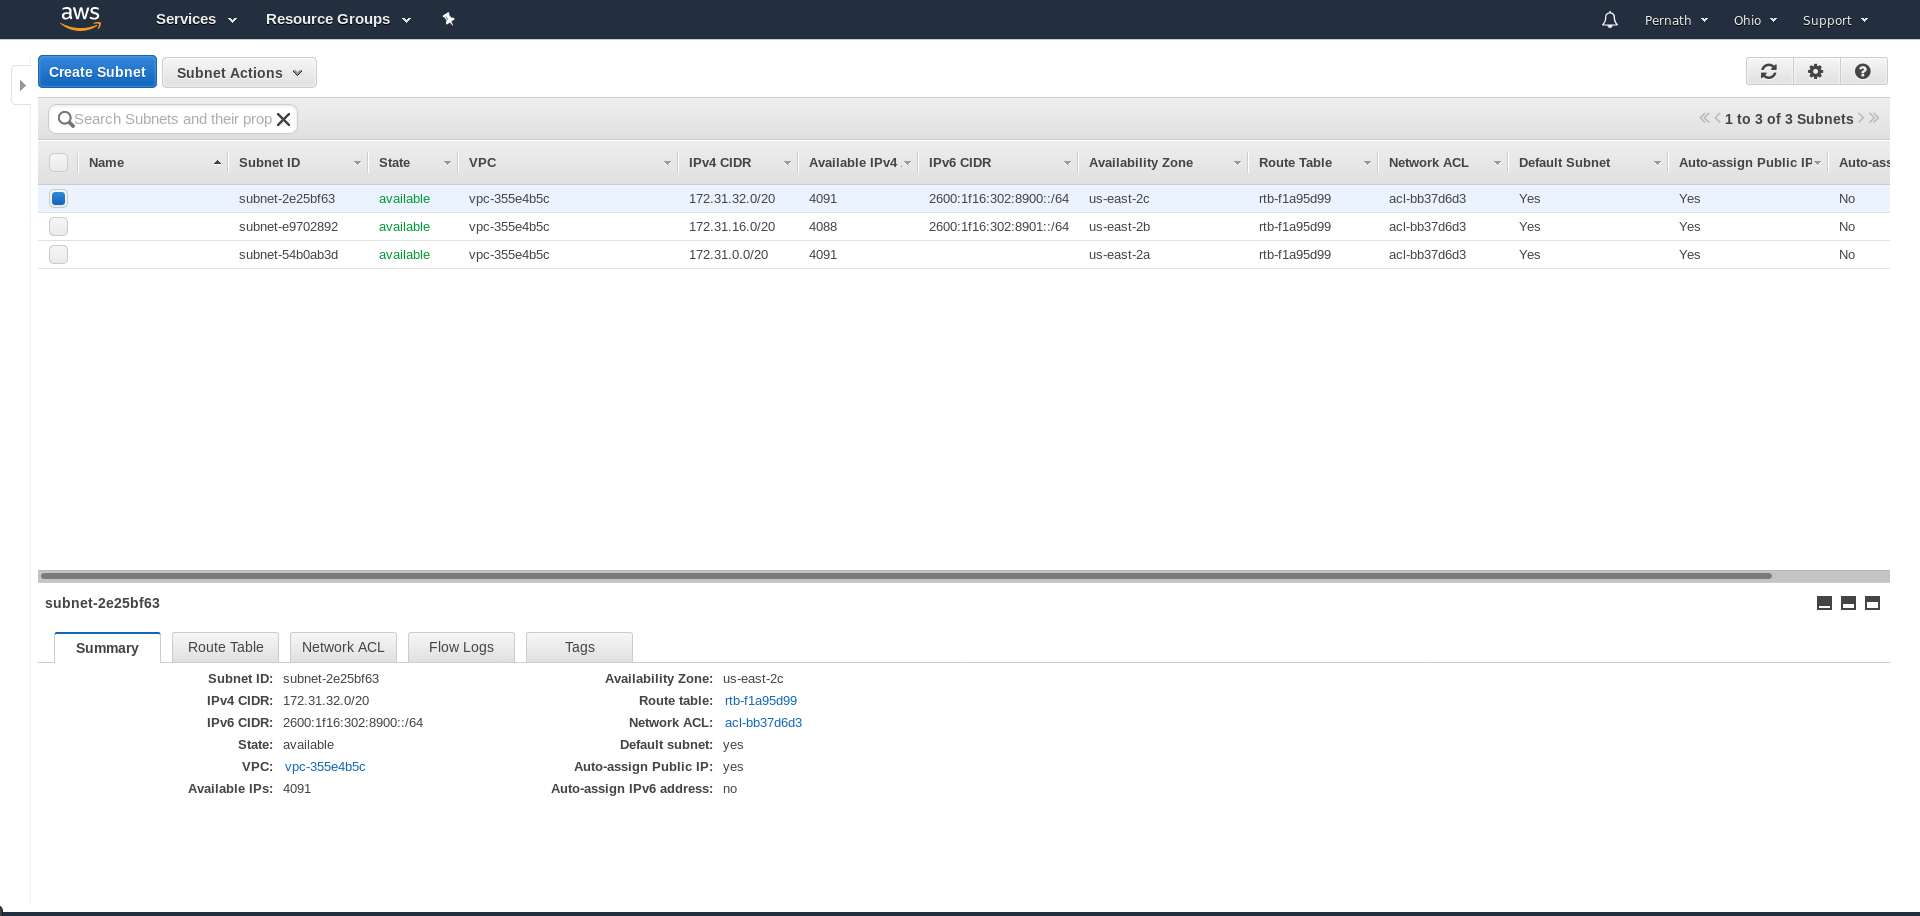
\includegraphics[width=\textwidth]{subnets}
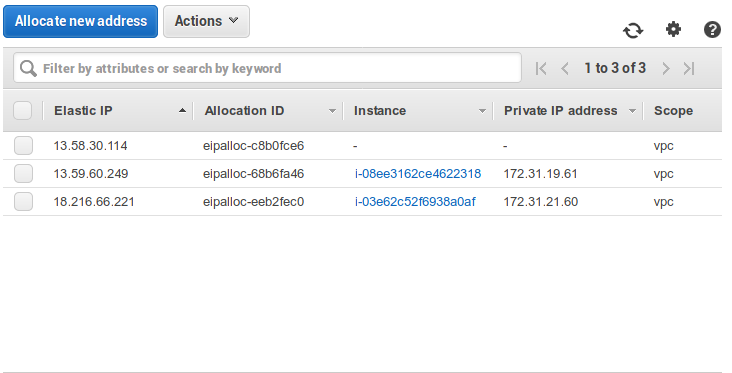
\includegraphics[width=\textwidth]{elastic_ip}
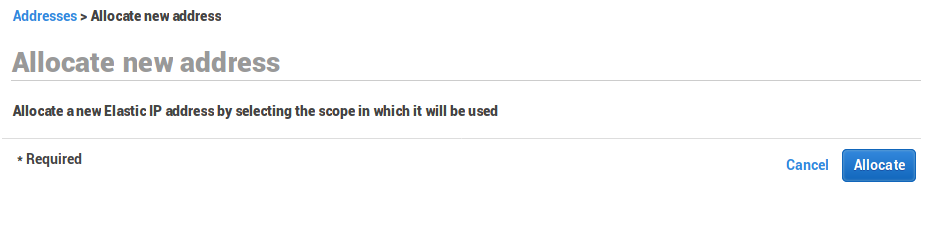
\includegraphics[width=\textwidth]{elastic_ip_allocate}
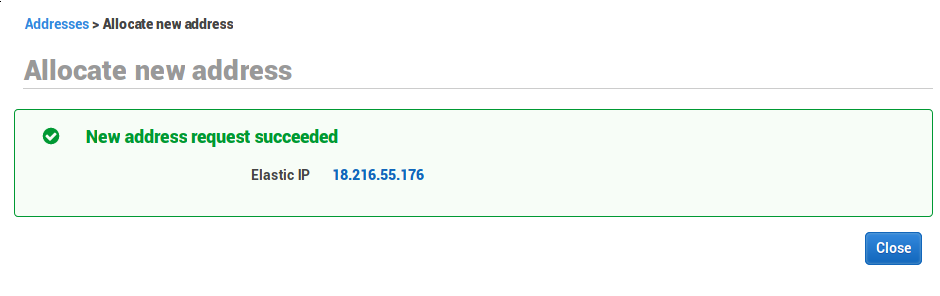
\includegraphics[width=\textwidth]{elastic_ip_success}
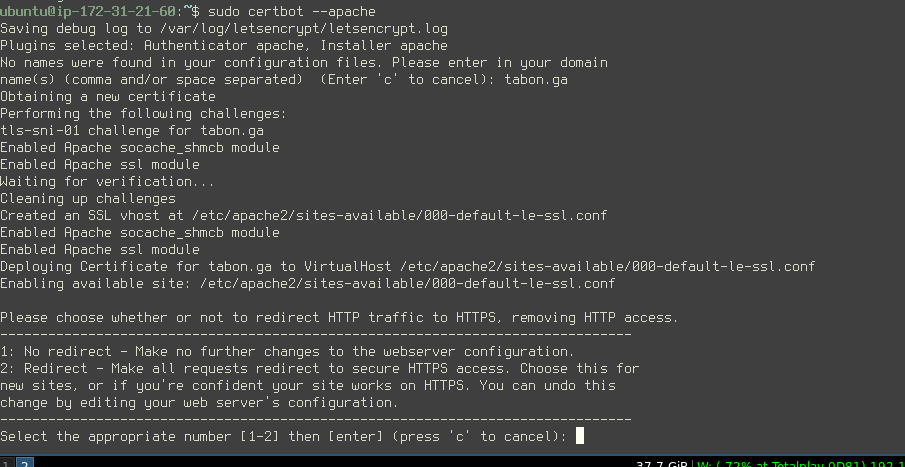
\includegraphics[width=\textwidth]{cert1}
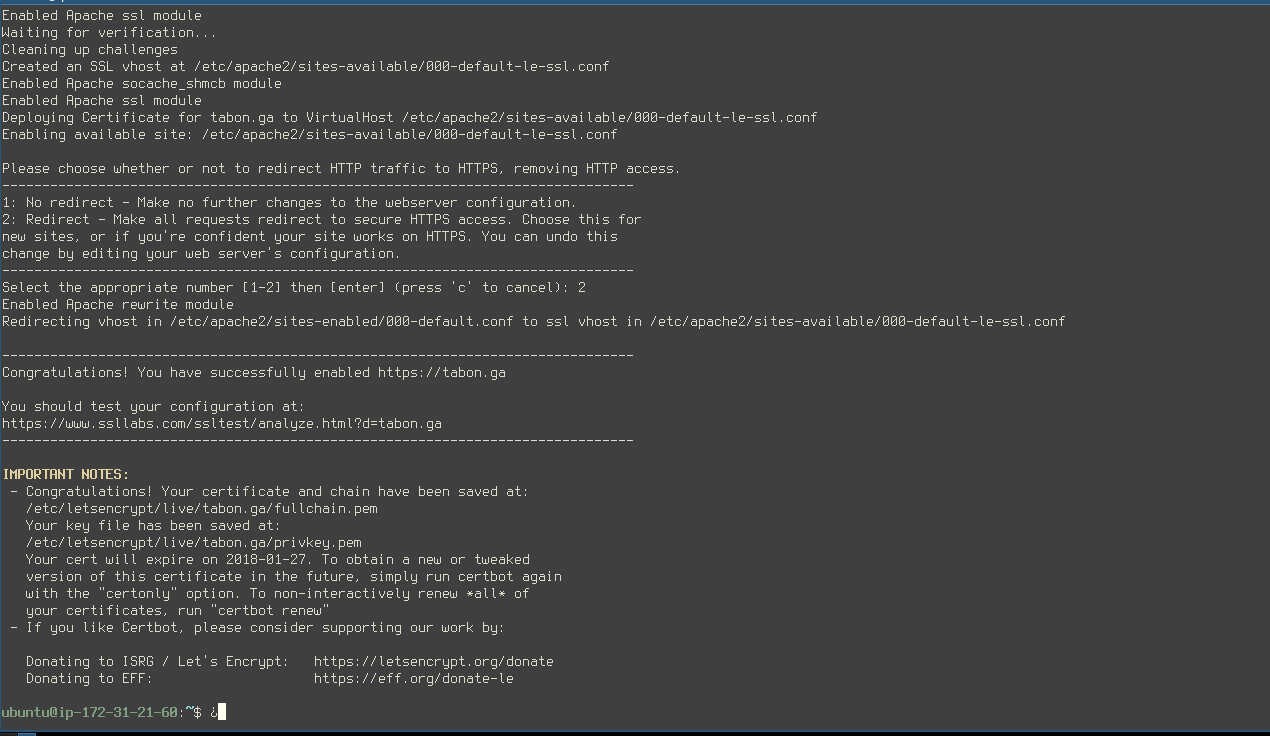
\includegraphics[width=\textwidth]{cert2}
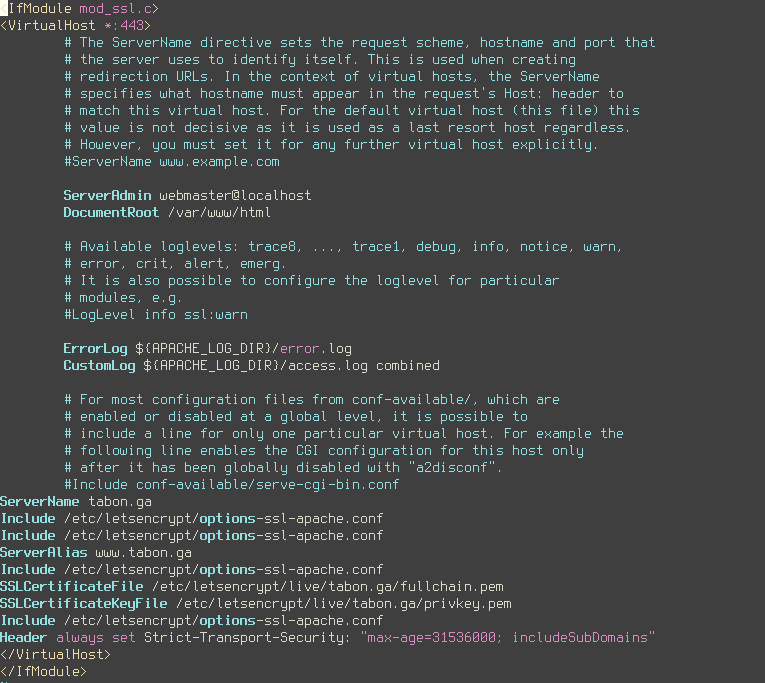
\includegraphics[width=\textwidth]{apache-ssl}
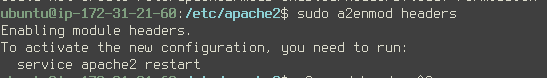
\includegraphics[width=\textwidth]{mods}
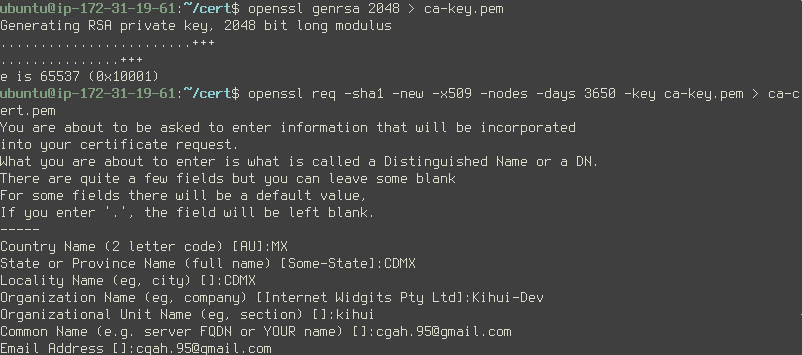
\includegraphics[width=\textwidth]{mysql_cert}
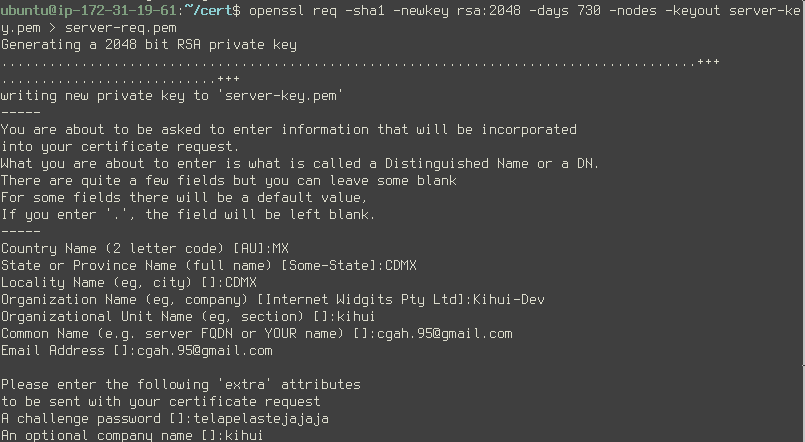
\includegraphics[width=\textwidth]{mysql_server-key}
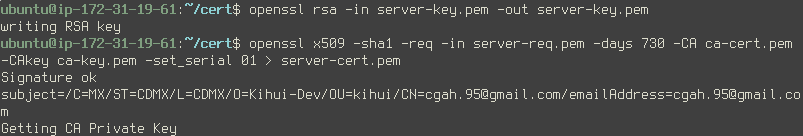
\includegraphics[width=\textwidth]{mysql_server-cert}
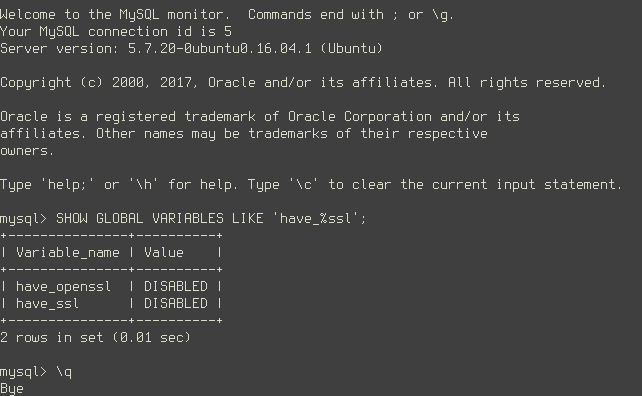
\includegraphics[width=\textwidth]{mysql_ssl-disabled}
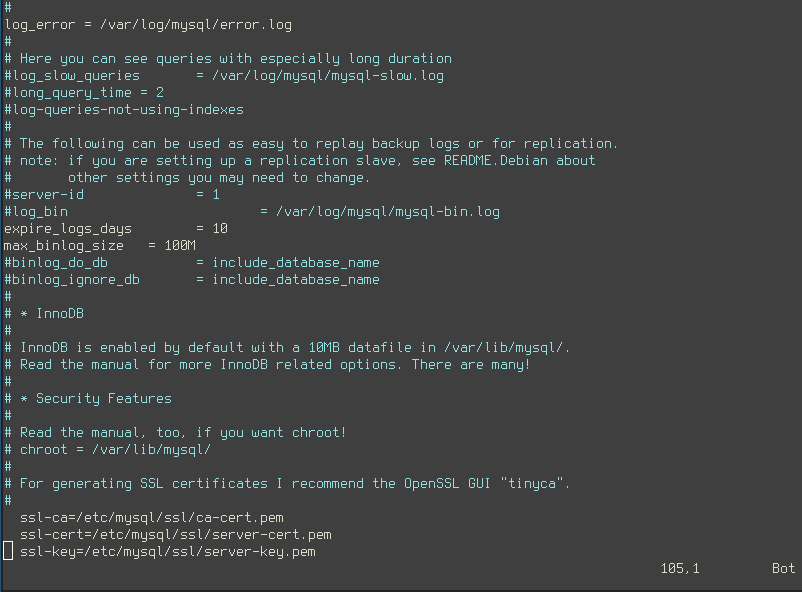
\includegraphics[width=\textwidth]{mysql_conf-ssl}
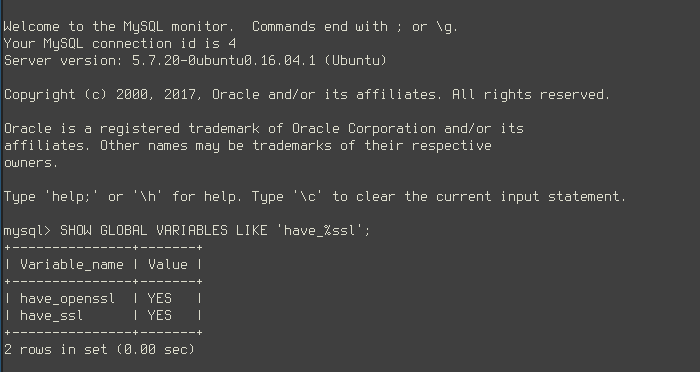
\includegraphics[width=\textwidth]{mysql_ssl-enabled}

\subsubsection*{Fail2ban}
Como los servidores tienen \textsf{Ubuntu} como sistema operativo, los archivos para la instalación de \textsf{fail2ban} están en los repositorios oficiales de la distribución, por lo que solo hizo falta ejecutar las instrucciones
\begin{verbatim}
# apt-get update
# apt-get install fail2ban
\end{verbatim}
Después de haber instalado \textsf{fail2ban} en el servidor, por recomendación de los desarrolladores, creamos un archivo \texttt{jail.local} como copia del archivo \texttt{jail.conf} que está en el directorio \texttt{/etc/fail2ban/} creado durante la instalación. En este archivo, habilitamos las \textit{jails} para restringir conexiones no autorizadas por fuerza bruta en los servicios de \textsf{ssh} y \textsf{apache} como se muestra a continuación:

\begin{figure}[H]
  \centering
  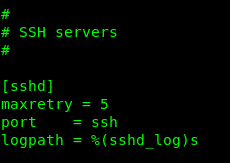
\includegraphics[scale=0.7]{fail2ban/ssh_jail}
  \caption{Configuración de jail para el servicio de ssh}
\end{figure}
\begin{figure}[H]
  \centering
  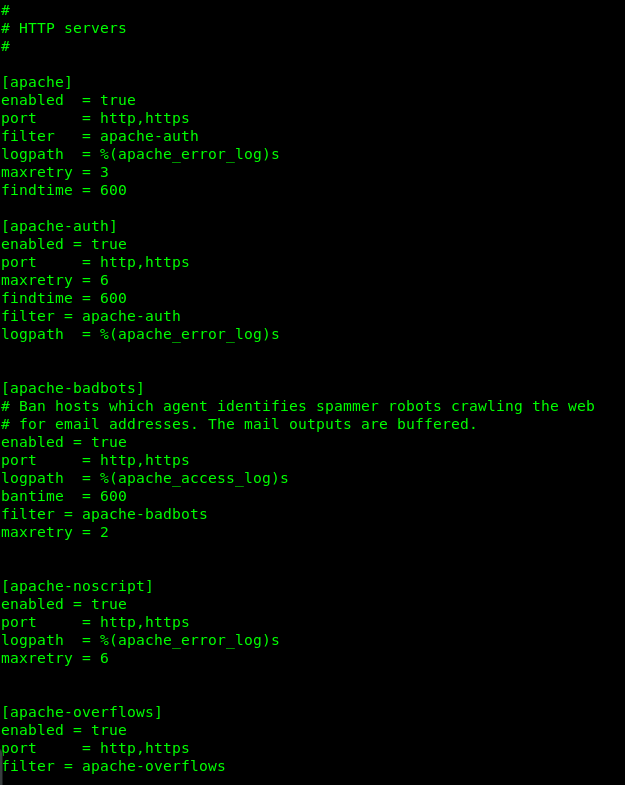
\includegraphics[scale=0.3]{fail2ban/apache_jails}
  \caption{configuración de jail para Apache}
\end{figure}

Para probar el funcionamiento de \textsf{fail2ban} se hicieron pruebas con distintas herramientas, como los \textit{benchmarks} de Apache, y verificamos el estado de las \textsf{iptables} antes y después de tales pruebas.
\begin{figure}[H]
  \centering
  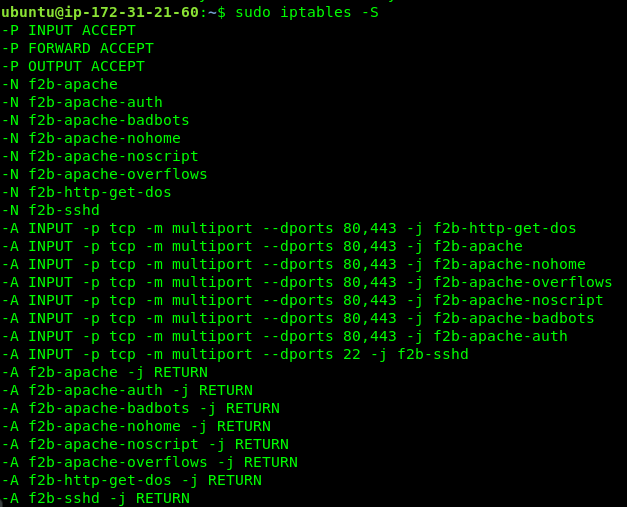
\includegraphics[scale=0.3]{fail2ban/iptables}
  \caption{estado de iptables después de configurar fail2ban}
\end{figure}
\begin{figure}[H]
  \centering
  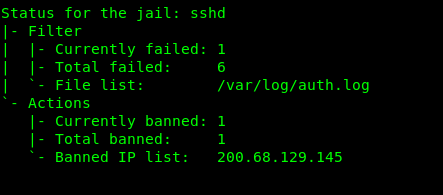
\includegraphics[scale=0.5]{fail2ban/ssh_banned_experiment}
  \caption{resultado de las pruebas para ssh}
\end{figure}
\begin{figure}[H]
  \centering
  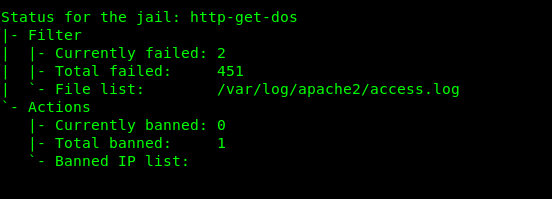
\includegraphics[scale=0.5]{fail2ban/fakeddos_test}
  \caption{resultado de una prueba de ataque DDoS}
\end{figure}
\begin{figure}[H]
  \centering
  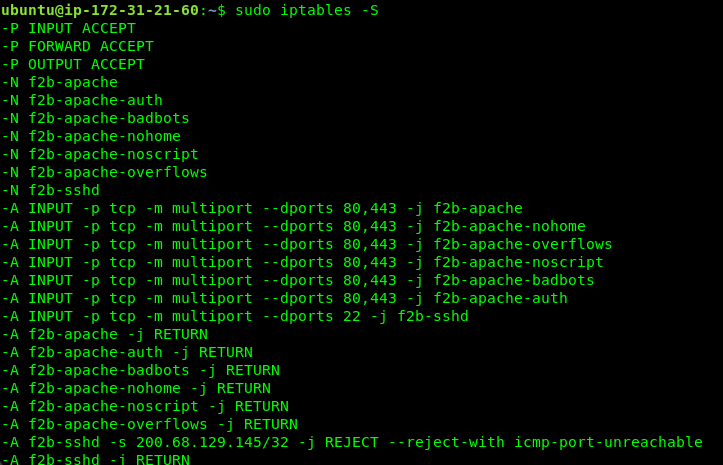
\includegraphics[scale=0.3]{fail2ban/new_iptables_with_ban}
  \caption{estado de iptables después de las pruebas}
\end{figure}
\vspace{2cm} %it just works
\subsection*{Diagrama de la base de datos}
Dada la simpleza de la aplicación, la base de datos solo cuenta con una tabla para los usuarios con sus respectivos atributos.\\
\begin{figure}[H]
  \centering
  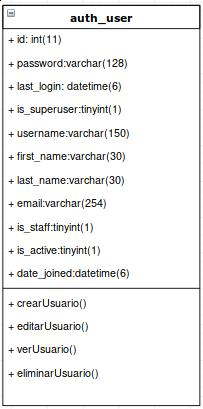
\includegraphics[scale=0.5]{db}
  \caption{Tabla de usuario}
\end{figure}

\subsection*{Objetivo de la aplicación}
La aplicación fue desarrollada con el fin de ilustrar las funciones básicas de una aplicación web con base de datos, es decir, \textit{crear, editar, ver y liminar} y que pueden asociarse a distintos métodos \textsf{HTTP} de la capa de aplicación como \textsf{PUT, POST, GET, PATCH o DELETE}. \\
A partir de esta pequeña aplicación \textit{CRUD} puede escalarse a proyectos más grandes y de mayor complejidad gracias a la escalabilidad de \textbf{Django}, el framework usado.

\subsection*{Uso de la aplicación}
Al ingresar al sitio, el usuario se encontrará con dos enlaces: uno para registrarse en la plataforma y otro para iniciar sesión en ésta.
\begin{figure}[h!]
  \centering
  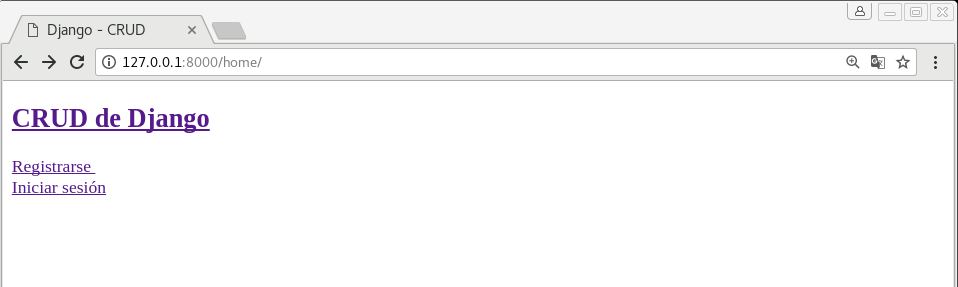
\includegraphics[width=\textwidth]{django_crud/home_notlogged}
  \caption{Página de inicio para usuarios sin sesión activa}
\end{figure}
\\
Si no está registrado e ingresa en el enlace para registrarse, será redireccionado a un formulario para que llene sus datos y se de de alta en la aplicación. 
\begin{figure}[h!]
  \centering
  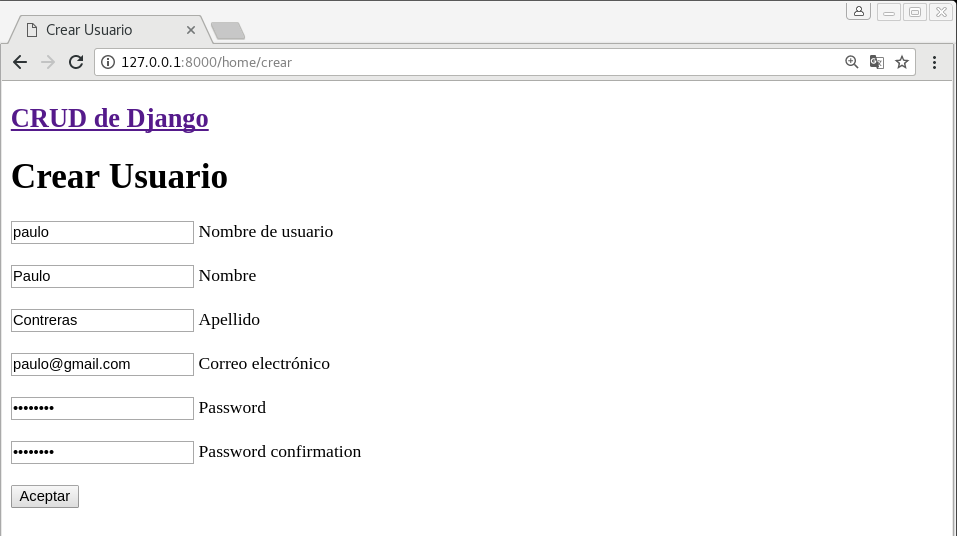
\includegraphics[width=\textwidth]{django_crud/registration}
  \caption{Formulario de registro para usuarios}
\end{figure}
\\
Si ya está registrado, podrá ingresar a la aplicación siguiendo el enlace de \textit{Iniciar sesión} en la página de inicio y en el formulario escribir el nombre de usuario y la contraseña con los que se registró.
\begin{figure}[h!]
  \centering
  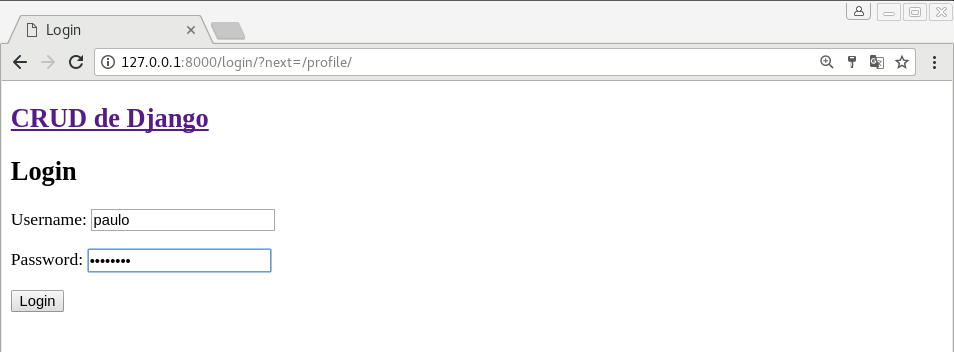
\includegraphics[width=\textwidth]{django_crud/login}
  \caption{Formulario de inicio de sesión}
\end{figure}
\\

Una vez dentro de la aplicación, el usuario verá una lista de los usuarios registrados y tendrá las opciones de ver información más detallada sobre algún usuario o sí mismo, actualizar sus datos o eliminar su cuenta si así lo desea.\\
\begin{figure}[ht!]
  \centering
  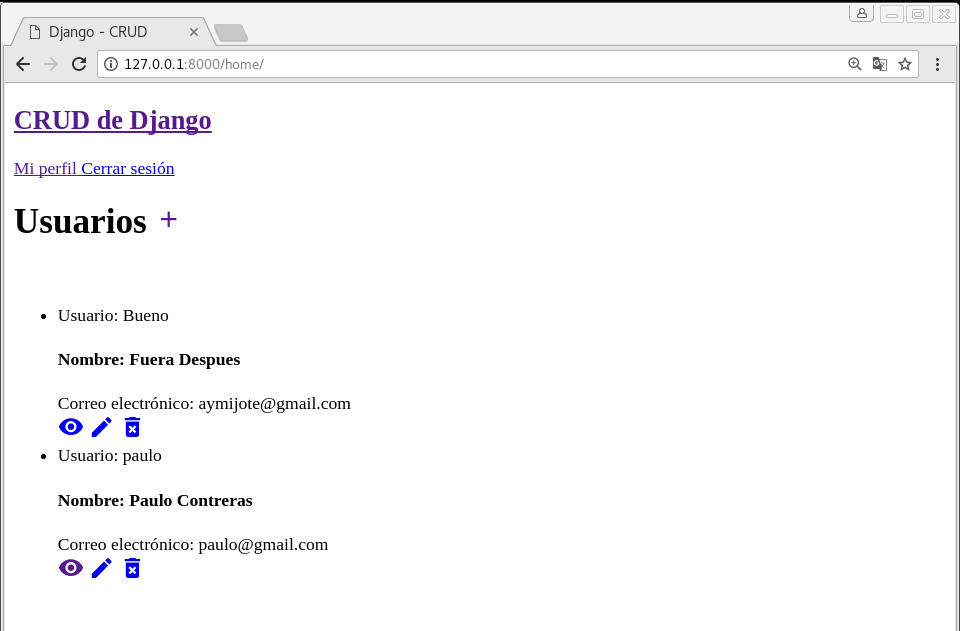
\includegraphics[width=\textwidth]{django_crud/home_logged}
  \caption{Página de inicio para usuarios con sesión activa}
\end{figure}
\\

Si elige ver información más detallada sobre un usuario, el enlace lo llevará al perfil del usuario. \\
\begin{figure}[ht!]
  \centering
  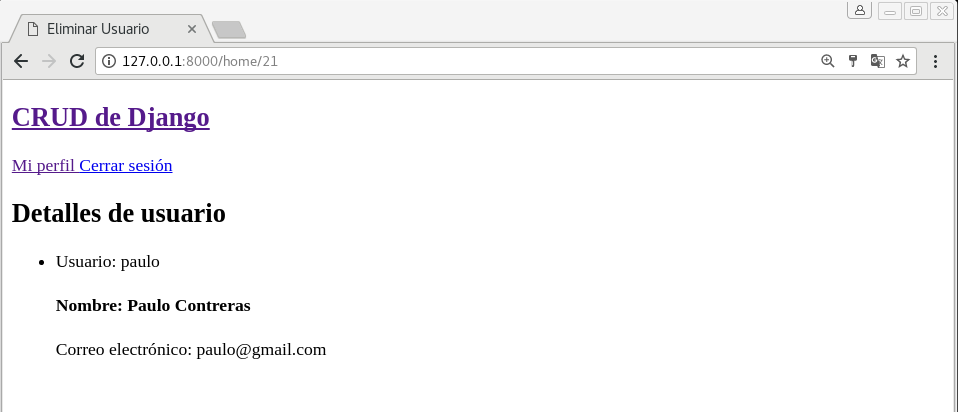
\includegraphics[width=\textwidth]{django_crud/profile}
  \caption{Perfil de usuario}
\end{figure}
\\

Para actualizar sus datos, será redirigido a un formulario similar al de registro.\\
\begin{figure}[ht!]
  \centering
  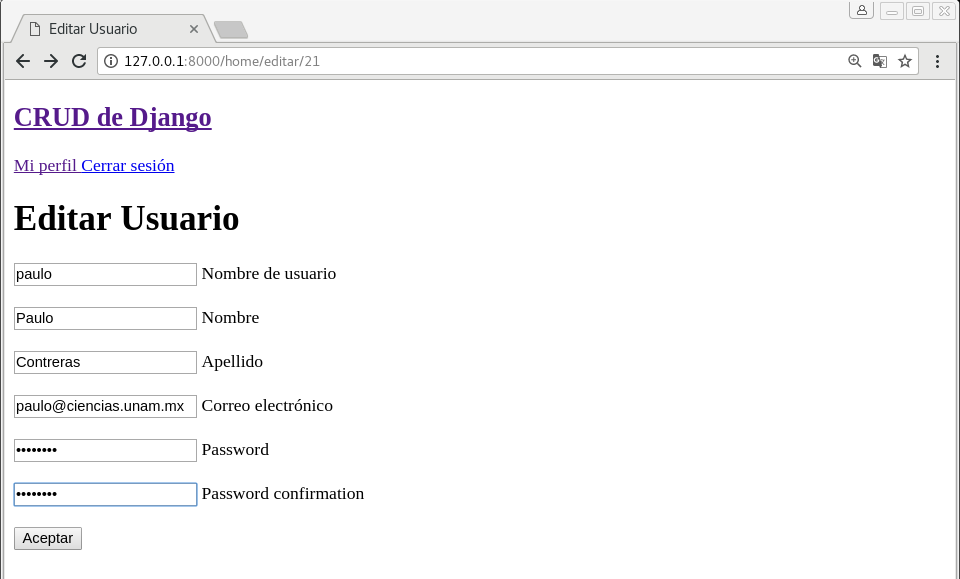
\includegraphics[width=\textwidth]{django_crud/update}
  \caption{Formulario de actualización de datos}
\end{figure}
\\

Si quiere eliminar su cuenta se le enviará un mensaje para que confirme su acción. \\
\begin{figure}[ht!]
  \centering
  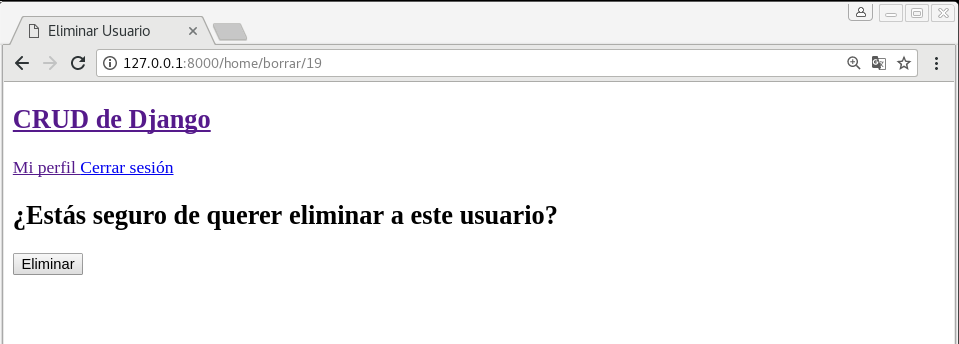
\includegraphics[width=\textwidth]{django_crud/delete}
  \caption{Mensaje de confirmación de eliminación de un usuario}
\end{figure}

\subsection*{Servidor de correos}

Utilizamos una máquina virtual con Ubuntu 16.04. Registramos el nombre de dominio \texttt{mail.tabon.ga} para su dirección IP correspondiente, que en este caso es la \texttt{13.58.30.114}. \\
Para el funcionamiento del servidor de correos utilizamos los paquetes de \texttt{postfix}, \texttt{dovecot}, \texttt{squirrelmail} y \texttt{apache2}. Tales paquetes se instalaron de la siguiente manera: \\
\begin{verbatim}
    $ sudo apt install postfix
    $ sudo apt install dovecot-core dovecot-imapd
    $ sudo apt install apache2
\end{verbatim}

\subsubsection*{letsencrypt}

Se instaló el bot de \textsf{letsencrypt}.
\begin{verbatim}
    $ sudo apt-get install software-properties-common
    $ sudo add-apt-repository ppa:certbot/certbot
    $ sudo apt-get update
    $ sudo apt-get install python-certbot-apache 
\end{verbatim}
Y se corrió con \texttt{sudo certbot --apache certonly}, al terminar creó la llave y certificados. \\
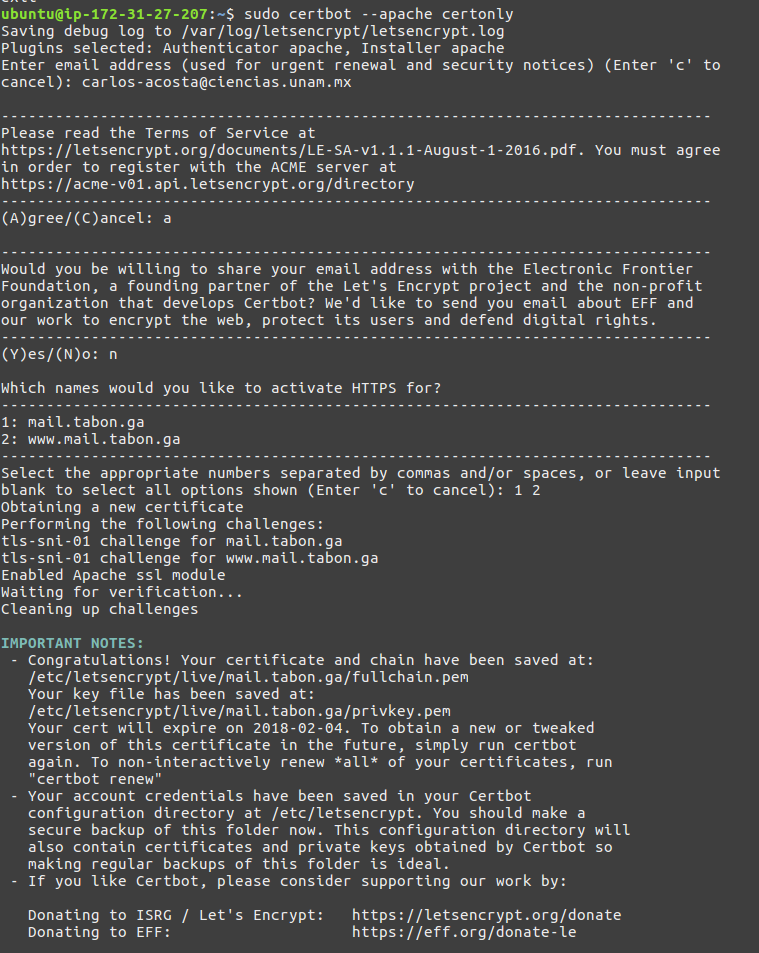
\includegraphics[scale=0.3]{mail/2}

\subsubsection*{Configuración de Postfix}
En el archivo \texttt{/etc/postfix/main.cf} se configuró lo siguiente:
\begin{verbatim}
smtpd_banner = $myhostname ESMTP $mail_name         
biff = no
append_dot_mydomain = no
readme_directory = no
smtpd_use_tls = yes
smtpd_tls_key_file = /etc/letsencrypt/live/mail.tabon.ga/privkey.pem
smtpd_tls_cert_file = /etc/letsencrypt/live/mail.tabon.ga/fullchain.pem
smtpd_tls_loglevel = 3
smtpd_tls_received_header = yes
smtpd_tls_session_cache_timeout = 3600s
tls_random_source = dev:/dev/urandom
smtpd_relay_restrictions = permit_mynetworks permit_sasl_authenticated \
                    defer_unauth_destination
myhostname = mail.tabon.ga                              
mydomain = tabon.ga
myorigin = /etc/mailname
mydestination = $myhostname, localhost.$mydomain, localhost, $mydomain
relayhost = 
mynetworks = 127.0.0.0/8, $mydomain, 132.247.0.0/16, 132.248.0.0/16
recipient_delimiter = +
inet_interfaces = all
inet_protocols = all
home_mailbox = mail/
smtpd_sasl_type = dovecot
\end{verbatim}
Se especificó donde se encuentra el certificado y llaves generados por \textsf{letsencrypt}, se modificó el banner de \texttt{smtp} y se pusieron restricciones de relay. \\
En el archivo \texttt{/etc/postfix/master.cf} se agregó lo siguiente:
\begin{verbatim}
smtp      inet  n       -       y       -       -       smtpd
submission inet n       -       y       -       -       smtpd
  -o smtpd_tls_security_level=encrypt
smtps     inet  n       -       y       -       -       smtpd
  -o smtpd_tls_wrappermode=yes
\end{verbatim}
de manera que se habilitara \texttt{smtps} y se abriera el puerto correspondiente (el 465). Finalmente se reinició el servicio con
\begin{verbatim}
    $ sudo systemctl restart postfix
\end{verbatim}

\subsubsection*{Configuración de Dovecot}

Se modificó el archivo \texttt{/etc/dovecot/dovecot.conf} con la siguiente línea:
\begin{verbatim}
listen = *, ::
\end{verbatim}

En \texttt{/etc/dovecot/conf.d/10-auth.conf} se agregó:
\begin{verbatim}
disable_plaintext_auth = yes
auth_mechanisms = plain login
\end{verbatim}

En \texttt{/etc/dovecot/conf.d/10-mail.conf}:
\begin{verbatim}
mail_location = maildir:~/mail
\end{verbatim}

Y en \texttt{/etc/dovecot/conf.d/10-ssl.conf}
\begin{verbatim}
ssl = yes
ssl_cert = </etc/letsencrypt/live/mail.tabon.ga/fullchain.pem
ssl_key = </etc/letsencrypt/live/mail.tabon.ga/privkey.pem
\end{verbatim}

\subsubsection*{Configuración de Squirrelmail}
Se corrió el bot de configuración de Squirrelmail:
\begin{verbatim}
    $ sudo squirrelmail-configure
\end{verbatim}

Por lo que se mostró el menú de configuración:

\begin{verbatim}
SquirrelMail Configuration : Read: config.php (1.4.0)
---------------------------------------------------------
Main Menu --
1.  Organization Preferences
2.  Server Settings
3.  Folder Defaults
4.  General Options
5.  Themes
6.  Address Books
7.  Message of the Day (MOTD)
8.  Plugins
9.  Database
10. Languages

D.  Set pre-defined settings for specific IMAP servers

C   Turn color on
S   Save data
Q   Quit

Command >> 
\end{verbatim}

Se seleccionó la opción 2. Se procedió a configurar las opciones de SMTP e IMAP, que quedaron de ka siguiente manera:

\begin{verbatim}
SquirrelMail Configuration : Read: config.php (1.4.0)
---------------------------------------------------------
Server Settings

General
-------
1.  Domain                 : tabon.ga
2.  Invert Time            : false
3.  Sendmail or SMTP       : SMTP

IMAP Settings
--------------
4.  IMAP Server            : mail.tabon.ga
5.  IMAP Port              : 993
6.  Authentication type    : login
7.  Secure IMAP (TLS)      : true
8.  Server software        : dovecot
9.  Delimiter              : /

SMTP Settings
-------------
4.   SMTP Server           : mail.tabon.ga
5.   SMTP Port             : 465
6.   POP before SMTP       : false
7.   SMTP Authentication   : none
8.   Secure SMTP (TLS)     : true
9.   Header encryption key : 
\end{verbatim}

% | egrep -v "(.*#.*|^$)"

\subsubsection*{Configuración de Apache}

Se habilitaron los modulos necesarios para que \texttt{https} funcione \\
\begin{verbatim}
    $ sudo a2enmod ssl
    $ sudo a2enmod headers
    $ sudo a2enmod rewrite
\end{verbatim}

Se copió el archivo de squirrelmail de apache a los sitios disponibles de apache, se habilitó junto con \texttt{default-ssl} y se deshabilitó el sitio por defecto de Apache. \\
\begin{verbatim}
sudo cp /etc/squirrelmail/apache.conf /etc/apache2/sites-available/squirrelmail.conf
sudo a2ensite squirrelmail.conf
sudo a2ensite default-ssl
sudo a2dissite 000-default.conf
\end{verbatim}

En el archivo \texttt{/etc/apache2/conf-enabled/security.conf} se modificó la firma de Apache para que no muestre su versión y el sistema operativo en uso. \\
\begin{verbatim}
ServerTokens Prod
ServerSignature Off
\end{verbatim}

El archivo \texttt{/etc/apache2/sites-available/squirrelmail.conf} quedó de la siguiente manera
\begin{verbatim}
Alias /mail /usr/share/squirrelmail
<Directory /usr/share/squirrelmail>
  Options FollowSymLinks
  <IfModule mod_php.c>
    php_flag register_globals off
  </IfModule>
  <IfModule mod_dir.c>
    DirectoryIndex index.php
  </IfModule>
  <Files configtest.php>
    order deny,allow
    deny from all
    allow from 127.0.0.1
  </Files>
</Directory>
RedirectMatch ^/$ /mail/
<IfModule mod_rewrite.c>
  <IfModule mod_ssl.c>
    <Location /squirrelmail>
      RewriteEngine on
      RewriteCond %{HTTPS} !^on$ [NC]
      RewriteRule . https://%{HTTP_HOST}%{REQUEST_URI}  [L]
    </Location>
  </IfModule>
</IfModule>
\end{verbatim}

El archivo \texttt{/etc/apache2/sites-available/default-ssl.conf} quedó de la siguiente manera:
\begin{verbatim}
<IfModule mod_ssl.c>
	<VirtualHost _default_:443>
		ErrorLog ${APACHE_LOG_DIR}/error.log
		CustomLog ${APACHE_LOG_DIR}/access.log combined
		SSLEngine on
		SSLCertificateFile	/etc/letsencrypt/live/mail.tabon.ga/fullchain.pem
		SSLCertificateKeyFile /etc/letsencrypt/live/mail.tabon.ga/privkey.pem
		<FilesMatch "\.(cgi|shtml|phtml|php)$">
				SSLOptions +StdEnvVars
		</FilesMatch>
		<Directory /usr/lib/cgi-bin>
				SSLOptions +StdEnvVars
		</Directory>
		ServerName mail.tabon.ga
		ServerAlias www.mail.tabon.ga
		Header always set Strict-Transport-Security "max-age=31536000; includeSubDomains; preload"
 
	</VirtualHost>
</IfModule>
\end{verbatim}

Al finalizar estas configuraciones se reiniciaron los servicios con \texttt{systemctl}. \\

Pudimos ver entonces la página de inicio de Squirrelmail al ingresar a \texttt{mail.tabon.ga}: \\
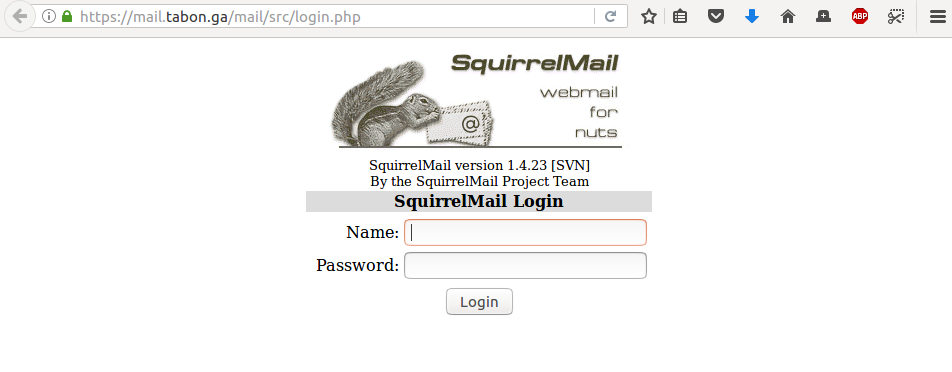
\includegraphics[scale=0.4]{mail/04} \\

Se agregaron los registros DNS de tipo MX y SPF para el dominio \texttt{tabon.ga} que son necesarios para el correcto funcionamiento del sistema, de manera que se acepte el correo que se manda al servidor asociado a tal dominio y se mande al servidor de correos, y que se evite que los correos mandados desde éste se vayan a spam. \\

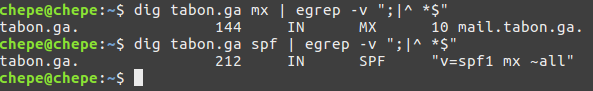
\includegraphics[scale=0.5]{mail/01} \\

Se cambió el puerto por defecto de ssh del 22 al 2200 y se definieron reglas de firewall desde la consola de AWS para sólo permitir los puertos necesarios: \\

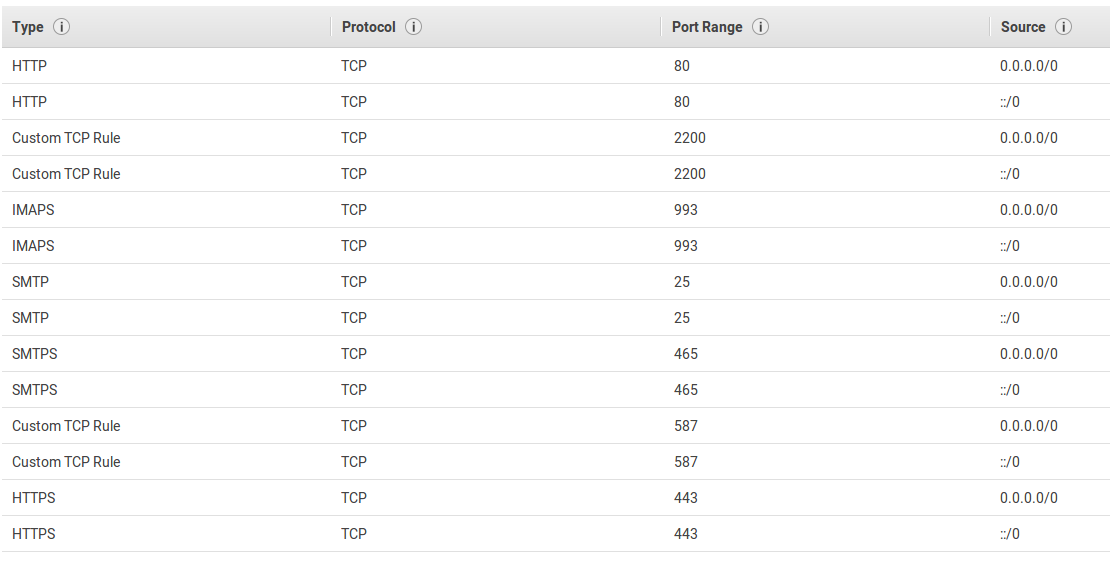
\includegraphics[scale=0.3]{mail/03} \\

\subsection*{Comentarios sobre el desarrollo del proyecto}
% We didn't deserve this
Intentamos hacer una aplicación lo más sencilla posible, minimizando la carga de trabajo que podría tener el servidor de aplicación, para enforcarnos en los aspectos más importantes que requería el proyecto: la comunicación entre los servidores y la seguridad en esta comunicación. %pero todo cambió cuando la nación del fuego atacó.

\end{document}
